%==============================================================================
% tento soubor pouzijte jako zaklad
% this file should be used as a base for the thesis
% Autoři / Authors: 2008 Michal Bidlo, 2019 Jaroslav Dytrych
% Kontakt pro dotazy a připomínky: sablona@fit.vutbr.cz
% Contact for questions and comments: sablona@fit.vutbr.cz
%==============================================================================
% kodovani: UTF-8 (zmena prikazem iconv, recode nebo cstocs)
% encoding: UTF-8 (you can change it by command iconv, recode or cstocs)
%------------------------------------------------------------------------------
% zpracování / processing: make, make pdf, make clean
%==============================================================================
% Soubory, které je nutné upravit nebo smazat: / Files which have to be edited or deleted:
%   projekt-20-literatura-bibliography.bib - literatura / bibliography
%   projekt-01-kapitoly-chapters.tex - obsah práce / the thesis content
%   projekt-01-kapitoly-chapters-en.tex - obsah práce v angličtině / the thesis content in English
%   projekt-30-prilohy-appendices.tex - přílohy / appendices
%   projekt-30-prilohy-appendices-en.tex - přílohy v angličtině / appendices in English
%==============================================================================
\documentclass[english]{fitthesis} % bez zadání - pro začátek práce, aby nebyl problém s překladem
%\documentclass[english]{fitthesis} % without assignment - for the work start to avoid compilation problem
%\documentclass[zadani]{fitthesis} % odevzdani do wisu a/nebo tisk s barevnými odkazy - odkazy jsou barevné
%\documentclass[english,zadani]{fitthesis} % for submission to the IS FIT and/or print with color links - links are color
%\documentclass[zadani,print]{fitthesis} % pro černobílý tisk - odkazy jsou černé
%\documentclass[english,zadani,print]{fitthesis} % for the black and white print - links are black
%\documentclass[zadani,cprint]{fitthesis} % pro barevný tisk - odkazy jsou černé, znak VUT barevný
%\documentclass[english,zadani,cprint]{fitthesis} % for the print - links are black, logo is color
% * Je-li práce psaná v anglickém jazyce, je zapotřebí u třídy použít 
%   parametr english následovně:
%   If thesis is written in English, it is necessary to use 
%   parameter english as follows:
%      \documentclass[english]{fitthesis}
% * Je-li práce psaná ve slovenském jazyce, je zapotřebí u třídy použít 
%   parametr slovak následovně:
%   If the work is written in the Slovak language, it is necessary 
%   to use parameter slovak as follows:
%      \documentclass[slovak]{fitthesis}
% * Je-li práce psaná v anglickém jazyce se slovenským abstraktem apod., 
%   je zapotřebí u třídy použít parametry english a enslovak následovně:
%   If the work is written in English with the Slovak abstract, etc., 
%   it is necessary to use parameters english and enslovak as follows:
%      \documentclass[english,enslovak]{fitthesis}

% Základní balíčky jsou dole v souboru šablony fitthesis.cls
% Basic packages are at the bottom of template file fitthesis.cls
% zde můžeme vložit vlastní balíčky / you can place own packages here

% Kompilace po částech (rychlejší, ale v náhledu nemusí být vše aktuální)
% Compilation piecewise (faster, but not all parts in preview will be up-to-date)
% \usepackage{subfiles}

% Nastavení cesty k obrázkům
% Setting of a path to the pictures
%\graphicspath{{obrazky-figures/}{./obrazky-figures/}}
%\graphicspath{{obrazky-figures/}{../obrazky-figures/}}

%---rm---------------
\renewcommand{\rmdefault}{lmr}%zavede Latin Modern Roman jako rm / set Latin Modern Roman as rm
%---sf---------------
\renewcommand{\sfdefault}{qhv}%zavede TeX Gyre Heros jako sf
%---tt------------
\renewcommand{\ttdefault}{lmtt}% zavede Latin Modern tt jako tt

% vypne funkci šablony, která automaticky nahrazuje uvozovky,
% aby nebyly prováděny nevhodné náhrady v popisech API apod.
% disables function of the template which replaces quotation marks
% to avoid unnecessary replacements in the API descriptions etc.
\csdoublequotesoff



\usepackage{url}


% =======================================================================
% balíček "hyperref" vytváří klikací odkazy v pdf, pokud tedy použijeme pdflatex
% problém je, že balíček hyperref musí být uveden jako poslední, takže nemůže
% být v šabloně
% "hyperref" package create clickable links in pdf if you are using pdflatex.
% Problem is that this package have to be introduced as the last one so it 
% can not be placed in the template file.
\ifWis
\ifx\pdfoutput\undefined % nejedeme pod pdflatexem / we are not using pdflatex
\else
  \usepackage{color}
  \usepackage[unicode,colorlinks,hyperindex,plainpages=false,pdftex]{hyperref}
  \definecolor{hrcolor-ref}{RGB}{223,52,30}
  \definecolor{hrcolor-cite}{HTML}{2F8F00}
  \definecolor{hrcolor-urls}{HTML}{092EAB}
  \hypersetup{
	linkcolor=hrcolor-ref,
	citecolor=hrcolor-cite,
	filecolor=magenta,
	urlcolor=hrcolor-urls
  }
  \def\pdfBorderAttrs{/Border [0 0 0] }  % bez okrajů kolem odkazů / without margins around links
  \pdfcompresslevel=9
\fi
\else % pro tisk budou odkazy, na které se dá klikat, černé / for the print clickable links will be black
\ifx\pdfoutput\undefined % nejedeme pod pdflatexem / we are not using pdflatex
\else
  \usepackage{color}
  \usepackage[unicode,colorlinks,hyperindex,plainpages=false,pdftex,urlcolor=black,linkcolor=black,citecolor=black]{hyperref}
  \definecolor{links}{rgb}{0,0,0}
  \definecolor{anchors}{rgb}{0,0,0}
  \def\AnchorColor{anchors}
  \def\LinkColor{links}
  \def\pdfBorderAttrs{/Border [0 0 0] } % bez okrajů kolem odkazů / without margins around links
  \pdfcompresslevel=9
\fi
\fi
% Řešení problému, kdy klikací odkazy na obrázky vedou za obrázek
% This solves the problems with links which leads after the picture
\usepackage[all]{hypcap}

% Informace o práci/projektu / Information about the thesis
%---------------------------------------------------------------------------
\projectinfo{
  %Prace / Thesis
  project={SP},            %typ práce BP/SP/DP/DR  / thesis type (SP = term project)
  year={2019},             % rok odevzdání / year of submission
  date=\today,             % datum odevzdání / submission date
  %Nazev prace / thesis title
  title.cs={Automatické generování testů pro GNOME GUI aplikace z metadat AT-SPI},  % název práce v češtině či slovenštině (dle zadání) / thesis title in czech language (according to assignment)
  title.en={Automated Generation of Tests for GNOME GUI Applications Using AT-SPI Metadata}, % název práce v angličtině / thesis title in english
  %title.length={14.5cm}, % nastavení délky bloku s titulkem pro úpravu zalomení řádku (lze definovat zde nebo níže) / setting the length of a block with a thesis title for adjusting a line break (can be defined here or below)
  %sectitle.length={14.5cm}, % nastavení délky bloku s druhým titulkem pro úpravu zalomení řádku (lze definovat zde nebo níže) / setting the length of a block with a second thesis title for adjusting a line break (can be defined here or below)
  %Autor / Author
  author.name={Martin},   % jméno autora / author name
  author.surname={Krajňák},   % příjmení autora / author surname 
  %author.title.p={Bc.}, % titul před jménem (nepovinné) / title before the name (optional)
  %author.title.a={Ph.D.}, % titul za jménem (nepovinné) / title after the name (optional)
  %Ustav / Department
  department={UITS}, % doplňte příslušnou zkratku dle ústavu na zadání: UPSY/UIFS/UITS/UPGM / fill in appropriate abbreviation of the department according to assignment: UPSY/UIFS/UITS/UPGM
  % Školitel / supervisor
  supervisor.name={Tomáš},   % jméno školitele / supervisor name 
  supervisor.surname={Vojnar},   % příjmení školitele / supervisor surname
  supervisor.title.p={prof. Ing.},   %titul před jménem (nepovinné) / title before the name (optional)
  supervisor.title.a={Ph.D.},    %titul za jménem (nepovinné) / title after the name (optional)
  % Klíčová slova / keywords
  keywords.cs={Sem budou zapsána jednotlivá klíčová slova v českém (slovenském) jazyce, oddělená čárkami.}, % klíčová slova v českém či slovenském jazyce / keywords in czech or slovak language
  keywords.en={Sem budou zapsána jednotlivá klíčová slova v anglickém jazyce, oddělená čárkami.}, % klíčová slova v anglickém jazyce / keywords in english
  %keywords.en={Here, individual keywords separated by commas will be written in English.},
  % Abstrakt / Abstract
  abstract.cs={Do tohoto odstavce bude zapsán výtah (abstrakt) práce v českém (slovenském) jazyce.}, % abstrakt v českém či slovenském jazyce / abstract in czech or slovak language
  abstract.en={Do tohoto odstavce bude zapsán výtah (abstrakt) práce v anglickém jazyce.}, % abstrakt v anglickém jazyce / abstract in english
  %abstract.en={An abstract of the work in English will be written in this paragraph.},
  % Prohlášení (u anglicky psané práce anglicky, u slovensky psané práce slovensky) / Declaration (for thesis in english should be in english)
  declaration={Prohlašuji, že jsem tuto bakalářskou práci vypracoval samostatně pod vedením pana X...
Další informace mi poskytli...
Uvedl jsem všechny literární prameny, publikace a další zdroje, ze kterých jsem čerpal.},
  %declaration={I hereby declare that this Bachelor's thesis was prepared as an original work by the author under the supervision of Mr. X
% The supplementary information was provided by Mr. Y
% I have listed all the literary sources, publications and other sources, which were used during the preparation of this thesis.},
  % Poděkování (nepovinné, nejlépe v jazyce práce) / Acknowledgement (optional, ideally in the language of the thesis)
  acknowledgment={V této sekci je možno uvést poděkování vedoucímu práce a těm, kteří poskytli odbornou pomoc
(externí zadavatel, konzultant apod.).},
  %acknowledgment={Here it is possible to express thanks to the supervisor and to the people which provided professional help
%(external submitter, consultant, etc.).},
  % Rozšířený abstrakt (cca 3 normostrany) - lze definovat zde nebo níže / Extended abstract (approximately 3 standard pages) - can be defined here or below
  %extendedabstract={Do tohoto odstavce bude zapsán rozšířený výtah (abstrakt) práce v českém (slovenském) jazyce.},
  %faculty={FIT}, % FIT/FEKT/FSI/FA/FCH/FP/FAST/FAVU/USI/DEF
  faculty.cs={Fakulta informačních technologií}, % Fakulta v češtině - pro využití této položky výše zvolte fakultu DEF / Faculty in Czech - for use of this entry select DEF above
  faculty.en={Faculty of Information Technology}, % Fakulta v angličtině - pro využití této položky výše zvolte fakultu DEF / Faculty in English - for use of this entry select DEF above
  department.cs={Ústav matematiky}, % Ústav v češtině - pro využití této položky výše zvolte ústav DEF nebo jej zakomentujte / Department in Czech - for use of this entry select DEF above or comment it out
  department.en={Institute of Mathematics} % Ústav v angličtině - pro využití této položky výše zvolte ústav DEF nebo jej zakomentujte / Department in English - for use of this entry select DEF above or comment it out
}

% Rozšířený abstrakt (cca 3 normostrany) - lze definovat zde nebo výše / Extended abstract (approximately 3 standard pages) - can be defined here or above
%\extendedabstract{Do tohoto odstavce bude zapsán výtah (abstrakt) práce v českém (slovenském) jazyce.}

% nastavení délky bloku s titulkem pro úpravu zalomení řádku - lze definovat zde nebo výše / setting the length of a block with a thesis title for adjusting a line break - can be defined here or above
%\titlelength{14.5cm}
% nastavení délky bloku s druhým titulkem pro úpravu zalomení řádku - lze definovat zde nebo výše / setting the length of a block with a second thesis title for adjusting a line break - can be defined here or above
%\sectitlelength{14.5cm}

% řeší první/poslední řádek odstavce na předchozí/následující stránce
% solves first/last row of the paragraph on the previous/next page
\clubpenalty=10000
\widowpenalty=10000

% checklist
\newlist{checklist}{itemize}{1}
\setlist[checklist]{label=$\square$}

\begin{document}
  % Vysazeni titulnich stran / Typesetting of the title pages
  % ----------------------------------------------
  \maketitle
  % Obsah
  % ----------------------------------------------
  \setlength{\parskip}{0pt}

  {\hypersetup{hidelinks}\tableofcontents}
  
  % Seznam obrazku a tabulek (pokud prace obsahuje velke mnozstvi obrazku, tak se to hodi)
  % List of figures and list of tables (if the thesis contains a lot of pictures, it is good)
  \ifczech
    \renewcommand\listfigurename{Seznam obrázků}
  \fi
  \ifslovak
    \renewcommand\listfigurename{Zoznam obrázkov}
  \fi
  % {\hypersetup{hidelinks}\listoffigures}
  
  \ifczech
    \renewcommand\listtablename{Seznam tabulek}
  \fi
  \ifslovak
    \renewcommand\listtablename{Zoznam tabuliek}
  \fi
  % {\hypersetup{hidelinks}\listoftables}

  \ifODSAZ
    \setlength{\parskip}{0.5\bigskipamount}
  \else
    \setlength{\parskip}{0pt}
  \fi

  % vynechani stranky v oboustrannem rezimu
  % Skip the page in the two-sided mode
  \iftwoside
    \cleardoublepage
  \fi

  % Text prace / Thesis text
  % ----------------------------------------------
  \ifenglish
    % This file should be replaced with your file with an thesis content.
%=========================================================================
% Authors: Michal Bidlo, Bohuslav Křena, Jaroslav Dytrych, Petr Veigend and Adam Herout 2019

\chapter{Introduction}
importance of GUI testing, goals, regressions, errors 

The goal of this work is to design and implement a tool for generating tests for GNOME desktop applications using AT-SPI metadata created as a by-product of an architecture supporting assistive technologies.

The architecture expose application as a tree of accessibility objects with their current state. Every object is defined by several properties and set of actions that can be invoked to change the current state. Since accessibility support has been implemented to very fundamental layers of GTK/GNOME framework (widget level), it provides a suitable way for development of automated test suites.\cite{pyatspi2} 

Modern GUI applications are being developed more rapidly with lack of proper regression testing. 

manual testing vs automation clanok

Additionally this effort should also help to reveal defects and missing parts in accessibility itself and improve the experience for users with disabilities.

\chapter{Accessibility}
Accessibility in general is a technology that helps people with disabilities to participate in essential life activities. Considering the accessibility as a part of GNOME desktop, it includes libraries and development tools allowing users with disabilities to use other options of interaction with GNOME desktop environment. Those options includes voice interfaces, screen readers and other alternative input devices.\cite{gnomeADG}
\section{The Accessibility Toolkit (ATK)}
Assistive technologies are receiving information from the Accessibility toolkit (ATK) which provides built-in API for all GNOME widgets. ATK provides a set of interfaces which are required to be implemented by GUI components. Therefore, assistive technologies are able to automatically read most of the labels on screen without any extra efforts made by developers. The interfaces are toolkit-independent, meaning that their implementation could be written for many widgets, including widgets from frameworks such as GTK\footnote{https://www.gtk.org/} and Qt\footnote{https://www.qt.io/}.
\section{GNOME Accessibility Implementation Library (GAIL)}
Majority of GNOME applications are written in GTK framework. The framework provides dynamically loadable module named GAIL implementing ATK interfaces for all GTK widgets. Once the module is loaded at runtime, the application is fully capable to cooperate with ATK without any further modifications.
GNOME desktop does not load accessibility support libraries by default, it has to be enabled by setting a special gsettings key which can be achieved either by dconf\footnote{https://wiki.gnome.org/Projects/dconf} editor or by execution of the \texttt{gsetting} command in terminal:
\begin{verbatim}
    gsettings get org.gnome.desktop.interface toolkit-accessibility true
\end{verbatim}
Additional configuration may be required for applications written in other frameworks such as QT or Java. Furthermore, implementations of other assitive technologies might be too application specific or use various techniques like OS event snooping etc. Compared to GNOME Desktop, all information required by assistive technologies (AT) are passed from GNOME Accessibility Framework to a toolkit-independent Service Provider Interface (SPI). The SPI is a key component providing stable and consistent API for screen readers, magnifiers, etc. Accessibility support is relying on per-toolkit implementation (GTK, QT, Java) and its APIs exported through relevant bridges to unified AT-SPI interface, as described on Diagram \ref{ATSPI_architecture}.

\begin{figure}[hbt]
	\centering
	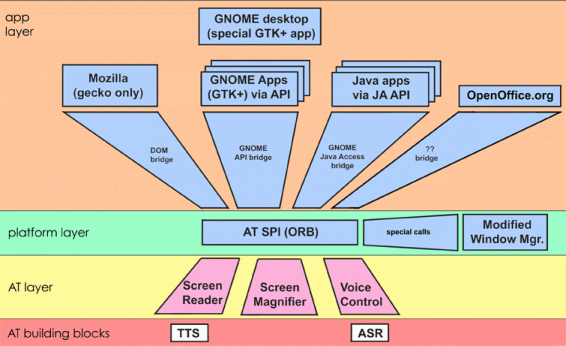
\includegraphics[width=1\textwidth]{obrazky-figures/GNOME_desktop_Accessibility.png}
	\caption{GNOME Accessibility Architecture overview}
	\label{ATSPI_architecture}
\end{figure}

The widget is accessible, if a developer use any GTK/GNOME widget and follows the general accessibility guidelines\footnote{https://developer.gnome.org/accessibility-devel-guide/stable/gad-coding-guidelines.html.en} with properly implemented ATK interfaces. Considering that the stock GTK/GNOME toolkit widgets have implementations of these interfaces provided, new widgets will inherit the functionality and gain suitable accessibility support as well. The default implementation of ATK interfaces might be altered by applications, as developers may improve their descriptions of widgets and improve the user experience in special cases when widget is used for some less expected purposes or the default description is too general. The ATK provides set of functions to achieve this along with the ability to make any custom component accessible\footnote{https://developer.gnome.org/accessibility-devel-guide/stable/gad-custom.html.en}.\cite{accessibleWidgets}

\newpage
\section{Library pyatspi}
Package pytaspi is a Python wrapper around AT-SPI C implementation which loads the Accessibility typelib and imports the classes implementing AT-SPI interfaces.\cite{pyatspi}

AT-SPI exposes applications as a tree of widgets starting with a root element where every sub-element represent one running application on the GNOME desktop. Each application has zero or more children, each child is distinguishable by its position in the tree and several properties including:
\begin{itemize}
    \item name - string value, for most widgets contains text identical with a text label visible on widget
    \item roleName - string value, specifies the widget type
    \item childCount - integer value, a number of sub-elements 
    \item actions - list of strings, contains available actions which can be performed by the ATK
    \item visible - boolean value, indicated that object is visible to the user
    \item showing - boolean value, object is rendered
    \item text - string value, mostly used in input fields or widgets containing plenty of text
    \item description - string value, contains special widget description for users
    \item position - integer tuple, x, y coordinates on the screen (might be related to other component)
\end{itemize}

Additionally, elements can be linked together in other useful ways (except parent-child relationship) where labels are linked with widgets like text fields, check boxes, combo boxes etc. These labels are making widgets easier to find or interact with. Other advantageous properties like showing or visible can be used to decide whether elements are hidden from the active screen area, thus they are not available for interaction. Role names of elements are also important as some elements are offering some widgets specific methods like selecting values in radio buttons, selecting options in combo boxes or a simple click method on push buttons. Access to this functionality is focused in a singleton object named registry that provides services for subscribing to specific events and as mentioned before, generating mouse and keyboard events on demand.

pyatspi is an open source project available for most of Linux distributions via distro specific packaging services (package named python3-atspi) or can be built from its sources\footnote{https://gitlab.gnome.org/GNOME/pyatspi2}.

\section{Expoloring and Debugging the Accesibility}
Currently, there are several tools available for exploration and debugging accessibility features not only on GNOME desktop. 
\subsection{dogtail}
Dogtail is an open source GUI test framework written in Python implemented as a library around pyatspi. Several modules implements another(higher) level of API to simplify work and interaction with accessible objects during test development. The tool offers less complex functionality, containing tree view of objects with their basic attributes\cite{dogtail_doc}. Dogtail package also includes a GUI tool Sniff, similar to the Accerciser application but described in the next section
The most important dogtail framework modules are:

\begin{itemize}
    \item tree - the module contains the most important class Node, instances of node class represent elements of the desktop user interface, all elements are gathered to tree structure representing all applications starting with the root element(desktop), the node class is implemented as a mixin for Accessible and various Accessible interfaces and is an important unit for it's subclasses, namely Application, Root and Window, the class also implements methods allowing to search for nodes in the tree based on certain criteria, including element properties name, rolename, showing and visible. Furthermore, it implements action methods that can be performed on the nodes without importing other modules, there is also a blink method, once it is called element is highlighted on the screen. This functionality is also part of the Sniff tool where element is highlighted after it is selected in the tree.    
    \item dump - dumping tree of nodes as a plain text, useful for python/ipython console debugging
    \item rawinput - contains implementation required for generating events from both keyboard and mouse, including more complex events like keyboard shortcut events and mouse gestures to emulate drag and drop operations  
\end{itemize}

 \begin{figure}[hbt]
	\centering
	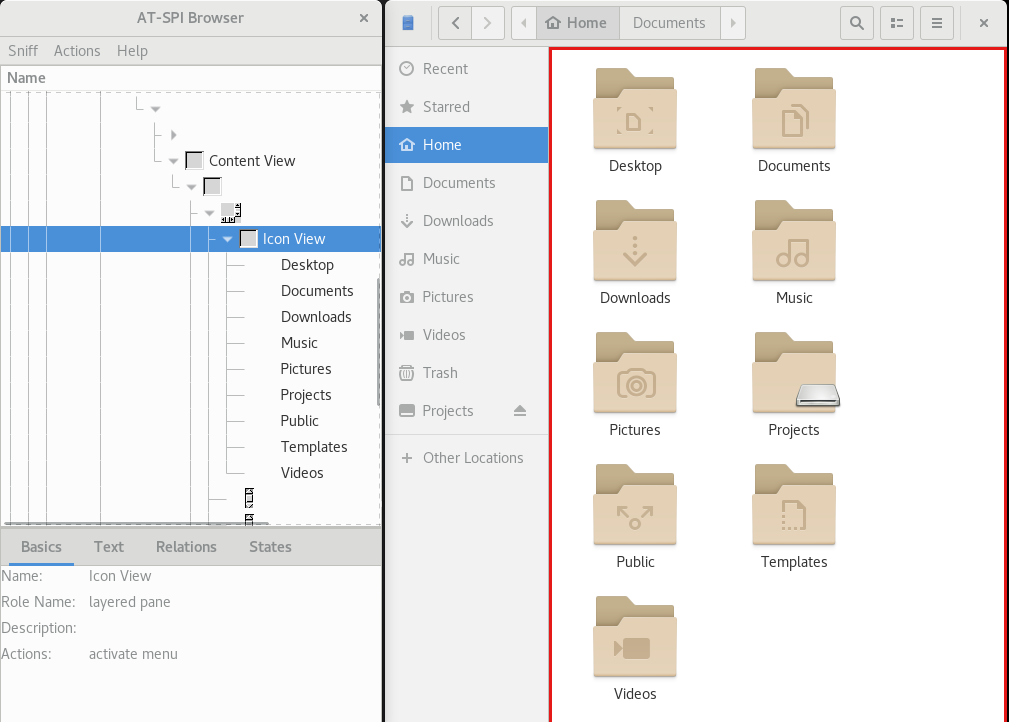
\includegraphics[width=1\textwidth]{obrazky-figures/sniff.png}
	\caption{Sniff utility highlighting icon area in Nautilus File Manager, Screenshot taken from Red Hat Enterprise Linux 8.2}
	\label{sniff}
\end{figure}

 Testing Dogtail has proven availability for many Linux distributions through their package repositories, specifically Fedora 32, Red Hat Enterprise Linux 8.2 and Manjaro 18 with GNOME 3.34 (Archlinux). It is also available as a Pypi Python package and according to information in it's official Gitlab repository should work not only for GTK+ application but also for application written in QT and KDE4. 
 
 Dogtail testing reveals also some minor problems which might occur during the test development, to be more specific the were cases when the coordinates of a node were not reported correctly. Some items are not labelled with names like panels and lists, those are mostly items that are not as important for user interaction as their are not containing any text but they are still accessible as they are parents for other elements of the UI. Unfortunately the testing discovered also some of the important buttons to be more specific menu buttons that are nameless. Once an action needs to be dispatched on such element it is required to use its parent or sibling element for identification and for actions performed by mouse make an adjustment of the coordinates, so it can be performed on the right node. So to conclude this chaper, dogtail is powerful tool for development of automated testing but it also has it's bug and limitations. Those limitations mustn't come from the dogtail itself but it might be caused either by accessibility bugs or just not respecting the accessibility guidelines during the development of the custom widgets. 

\subsection{Accerciser}
Accerciser is an interactive accessibility explorer developed in Python. It provides well-arranged graphical frontend for AT-SPI library, hence it can inspect, examine and interact with widgets and also allows developers to verify that their applications are providing correct information to assistive technologies and automated testing frameworks. The default interface has three sections: A tree view with the entire desktop accessible hierarchy and two optional plugin areas. Accerciser has an extensible, plugin-based architecture, most of the features available by default are part of the following plugins\cite{accerciser}: 

\begin{itemize}
    \item Interface Viewer - explorer of the AT-SPI interfaces provided by each accessible widget of a target application, after an item is selected, interfaces shown for the selected item will become sensitive, so all methods can be executed, including methods for object interaction like click and other methods for retrieving more object information. Accerciser allows to explore the following interfaces:
    \begin{itemize}
        \item Accessible - show child count (number of child widgets), description, states, relations and other attributes
        \item Application - if implemented (not mandatory), it shows application ID, toolkit and version
        \item Component - shows item's absolute position with respect to the desktop coordinate system, relative position with respect to the  window coordinate system, size, layer type, MDI-Z-order indicating the stacking order of the component and alpha
        \item Document - shows document attributes and locale information
        \item Hypertext - shows a list with all item's hypertext links,  including name, URI, start index and end index
        \item Image - shows item's description, size, position and locale
        \item Selection - shows all selectable child items of the selected item,
        \item Streamable Content - shows selected item's content type and their corresponding URIs
        \item Table - shows item's caption, rows, columns, number of selected rows, number of selected columns and for selected cell, it shows  it's row's and column's header extents  
        \item Text - shows selected item's text content, that can be editable with attributes offset, justification  and possibility to show CSS formatting as well
        \item Value shows item's value, minimum value, maximum value, minimal increment for a value 
    \end{itemize}
    \item AT-SPI Validator - applies tests to verify the accessibility of a target application, the validator will generate the report of the selected item and all its descendant widgets in the tree hierarchy
    \item Event Monitor - displays AT-SPI emitted events, it also provides the filter for several different AT-SPI event classes with the ability to monitor only events sourced from selected application or selected accessible(widget), each event record contains the source and the application.
    \item Quict Select - provides global hotkeys for quickly selecting accessible widgets in Accerciser's Application Tree View, selected widget is highlighted in the target application
    \item API Browser - shows interfaces, methods and attributes available on each accessible widgets of a target application, by default it shows only public methods and properties, private methods and properties are hidden until checkbox \texttt{Hide Private Attributes} is unchecked
    \item IPython Console - full, interactive Python shell with access to selected accessible widgets of a target application, use full debugging tool especially in combination with the Interface Viewer
\end{itemize}

\begin{figure}[hbt]
	\centering
	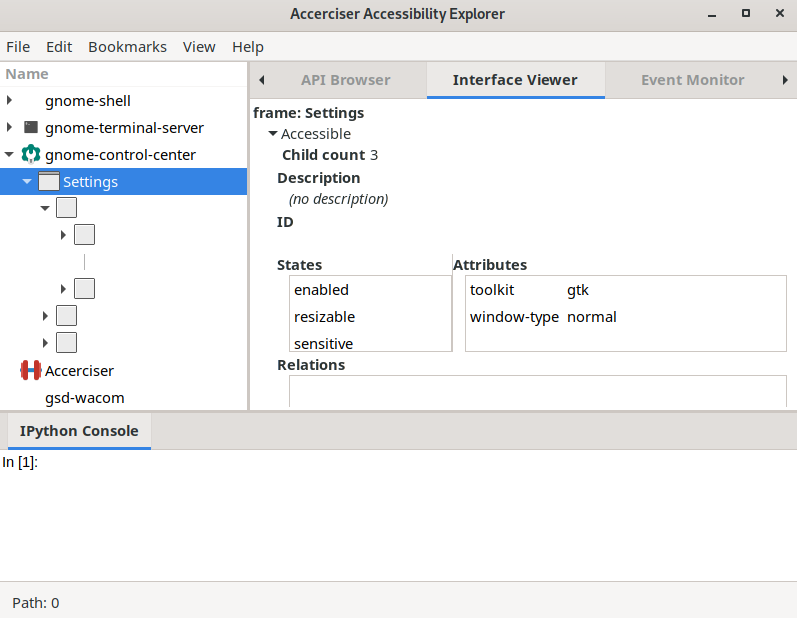
\includegraphics[width=1\textwidth]{obrazky-figures/accerciser.png}
	\caption{Accerciser default configuration, Screenshot taken on Manjaro Linux with GNOME 3.34}
	\label{Accerciser}
\end{figure}

\chapter{GUI TESTING}
https://ldtp.freedesktop.org/wiki/
https://en.wikipedia.org/wiki/Linux_Desktop_Testing_Project
https://wiki.ubuntu.com/Xpresser/
AppStream data
\chapter{python}
\chapter{behave}
\chapter{Verification}
As discussed in aforementioned chapters information provided by accessibility is not flawless, therefore next couple chapters are dedicated to exploration of technologies that might be used to support the accessibility in such cases.

\section{OpenCV2 - image comparison}
OpenCV or Open Source Computer Vision Library is a software library that provides optimized algorithms for computer vision and machine learning. According to official OpenCV webpage\cite{opencv}, the library contains more then 2500 algorithms and it is being developed 
by a vast community of contributors around the world. The library is used extensively bu government institutions, research groups and companies including Microsoft, Google, IBM and many more. One of the biggest advantages is its native C++ implementation with bindings making the library available in Python, Java and Matlab and supports Linux, Android, Mac OSX and Windows. Regardless of Linux distribution, similarly to dogtail, OpenCV can be installed easily via python3 package manager(pip). 

From the rich availability of algorithms provided, an image recognition algorithm can be used to either locate of verify the presence of an element on the screen. This approach would require to have and image of the element prepared in advance, then it can be used to find the image location on the screenshot of the screen taken during a test run. Compared to verification of the node only via accessibility, this approach would also verify that the element is properly rendering on screen and the shown result is really an element that has to be shown to the user with verification of text formatting and colors. On contrary, there this process requires additional manual work of taking images, labelling them and associating them with certain test scenarios. Additionally, more complications might appear as some of the elements may be displayed on the screen multiple times which would make a count of items on the screen at the same time another compulsory parameter that is required to maintain. The most common example of such case are buttons labelled either OK or Cancel as they are used in many applications.

Another possible approach is to use the shape recognition algorithm which can locate shapes like circles, rectangles any many other common shapes. From the development perspective this would be easier to maintain as there is no requirement for images prepared in advance(compared to image recognition algorithm) but can help with the widget location in cases where accessibility is reporting wrong coordinates. On the other hand, locating the right widget in cases when several similarly shaped ones are located on the screen at the same time will yield very inconsistent results.


\section{OCR text recognition pytesseract}

\begin{figure}[hbt]
	\centering
	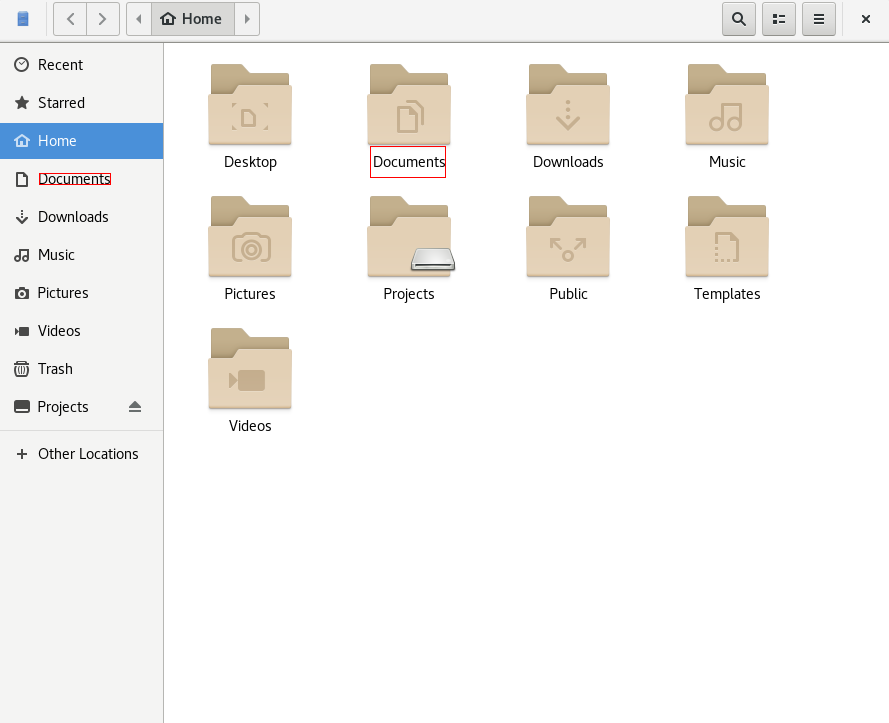
\includegraphics[width=1\textwidth]{obrazky-figures/ocr+nautilus.png}
	\caption{OCR detection of the Document string in Nautilus File Manager Window}
	\label{ocr_nautilus}
\end{figure}

\section{Conclusion}
  \else
    \input{projekt-01-kapitoly-chapters}
  \fi
  
  % Kompilace po částech (viz výše, nutno odkomentovat)
  % Compilation piecewise (see above, it is necessary to uncomment it)
  %\subfile{projekt-01-uvod-introduction}
  % ...
  %\subfile{chapters/projekt-05-conclusion}


  % Pouzita literatura / Bibliography
  % ----------------------------------------------
\ifslovak
  \makeatletter
  \def\@openbib@code{\addcontentsline{toc}{chapter}{Literatúra}}
  \makeatother
  \bibliographystyle{bib-styles/Pysny/skplain}
\else
  \ifczech
    \makeatletter
    \def\@openbib@code{\addcontentsline{toc}{chapter}{Literatura}}
    \makeatother
    \bibliographystyle{bib-styles/Pysny/czplain}
  \else 
    \makeatletter
    \def\@openbib@code{\addcontentsline{toc}{chapter}{Bibliography}}
    \makeatother
    \bibliographystyle{bib-styles/Pysny/enplain}
  %  \bibliographystyle{alpha}
  \fi
\fi
  \begin{flushleft}
  \bibliography{projekt-20-literatura-bibliography}
  \end{flushleft}

  % vynechani stranky v oboustrannem rezimu
  % Skip the page in the two-sided mode
  \iftwoside
    \cleardoublepage
  \fi

  % Prilohy / Appendices
  % ---------------------------------------------
  \appendix
\ifczech
  \renewcommand{\appendixpagename}{Přílohy}
  \renewcommand{\appendixtocname}{Přílohy}
  \renewcommand{\appendixname}{Příloha}
\fi
\ifslovak
  \renewcommand{\appendixpagename}{Prílohy}
  \renewcommand{\appendixtocname}{Prílohy}
  \renewcommand{\appendixname}{Príloha}
\fi
%  \appendixpage

% vynechani stranky v oboustrannem rezimu
% Skip the page in the two-sided mode
%\iftwoside
%  \cleardoublepage
%\fi
  
\ifslovak
%  \section*{Zoznam príloh}
%  \addcontentsline{toc}{section}{Zoznam príloh}
\else
  \ifczech
%    \section*{Seznam příloh}
%    \addcontentsline{toc}{section}{Seznam příloh}
  \else
%    \section*{List of Appendices}
%    \addcontentsline{toc}{section}{List of Appendices}
  \fi
\fi
  \startcontents[chapters]
  \setlength{\parskip}{0pt} 
  % seznam příloh / list of appendices
  % \printcontents[chapters]{l}{0}{\setcounter{tocdepth}{2}}
  
  \ifODSAZ
    \setlength{\parskip}{0.5\bigskipamount}
  \else
    \setlength{\parskip}{0pt}
  \fi
  
  % vynechani stranky v oboustrannem rezimu
  \iftwoside
    \cleardoublepage
  \fi
  
  % Přílohy / Appendices
  \ifenglish
    % % This file should be replaced with your file with an appendices (headings below are examples only)

% % Placing of table of contents of the memory media here should be consulted with a supervisor
% %\chapter{Contents of the included storage media}

% %\chapter{Manual}

% %\chapter{Configuration file}

% %\chapter{Scheme of RelaxNG configuration file}

% %\chapter{Poster}

% \chapter{How to use this template}
% \label{jak}

% This chapter describes individual parts of the template, followed by a brief instructions on how to use it. If you have any questions, comments etc, feel free to email them to \texttt{sablona@fit.vutbr.cz}.

% \section*{Template parts description}

% Once you extract the template, you will find the following files and directories:
% \begin{DESCRIPTION}
%   \item [bib-styles] Literature styles (see below). 
%   \item [obrazky-figures] Directory for your images. Currently contains \texttt{placeholder.pdf} (a.k.a TODO image -- see below) and image keep-calm.png to demonstrate inserting raster images (you don't submit these images with your thesis). It is advised to use shorter directory name, so that it is only in your chosen language.
%   \item [template-fig] Template images (BUT logo).
%   \item [fitthesis.cls] Template (design definition).
%   \item [Makefile] Makefile used to compile the project, count standard pages etc. (see below).
%   \item [projekt-01-kapitoly-chapters-en.tex] File for Your text (replace it's contents).
%   \item [projekt-20-literatura-bibliography.bib] Reference list (see below).
%   \item [projekt-30-prilohy-appendices-en.tex] File for your appendices (replace it's contents).
%   \item [projekt.tex] Main project file -- definitions of formal parts.
% \end{DESCRIPTION}

% The style of literature in the template is from Ing. Radek Pyšný \cite{Pysny}, whose work was improved by prof. Adam Herout, dr. Jaroslav Dytrych and Mr. Karel Hanák to comply with the norm and support all frequently used types of citations. Its documentation can be found in the appendix

% Aside from compilation to PDF, the Makefile also offers additional functions:
% \begin{itemize}
%   \item rename files (see below),
%   \item count standard pages,
%   \item run a wave that adds unbreakable spaces,
%   \item compress (zip) the result, ready to be sent to your supervisor and checked (make sure that all the files you've added are included, if not, add them manually).
% \end{itemize}

% Keep in mind that the wave is not perfect. You always need to check whether or not there is something inappropriate at the end of a line manually -- see Online language handbook\footnote{Internetová jazyková příručka \url{http://prirucka.ujc.cas.cz/?id=880}}.

% Similar rules apply also in English - see eg. article Run Ragged\footnote{Run Ragged\url{https://24ways.org/2013/run-ragged/}}, according to which there should be no prepositions, dash or short words (2--3 letters) at the end of the lines, the two lines following each other should not end with a comma and line break should not be also in the phrases from 2-3 words.

% \paragraph {Pay attention to page numbering!} If the table of contents is 2 pages long and the second page contains only \uv{Enclosures} and \uv{List of enclosures} (but there is no enclosure), the page numbering is changed by 1 (table of contents and contents \uv{mismatch}). The same thing happens if the second or third page contains only \uv{References} and there's a chance that this can occur in other situations too. There are multiple solutions to this (from editing the table of contents, setting the page counter all the way to more sophisticated methods). \textbf{Check the page numbering before you submit your thesis!}

% \section*{Recommendations for working with the template}

% \begin{enumerate}
%   \item \textbf{Make sure you have the latest version of template.} If you have a template from last year, there should be a newer version (updated information, fixed errors etc.) available at the faculty or study advisor web pages.  
%   \item \textbf{Choose a language}, that you want to use for your technical report (czech, slovak or english) and consult your supervisor about your choice (unless it was agreed upon in advance). If your language of choice is not czech, set the respective template parameter in file projekt.tex (e.g.: \verb|document|\verb|class[english]{fitthesis}| and translate the declaration and acknowledgement to english or slovak).
%   \item \textbf{Rename the files.} When you extract the files, there should be a file named projekt.tex. If you compile it, it will create a PDF with technical report named projekt.pdf. If multiple students send their supervisor projekt.pdf to have it checked, they have to rename them. For that reason, it is advised to rename the file so that it contains your login and (if needed, abbreviated) work topic. Avoid using spaces, diacritic and special symbols. An appropriate name for your file can look like this: \uv{xlogin00-Cleaning-and-extraction-of-text.tex}. You can use the included Makefile to rename it: 
% \begin{verbatim}
% make rename NAME=xlogin00-Cleaning-and-extraction-of-text
% \end{verbatim}
%   \item Fill in the required information in file, that was originally named projekt.text, that means type, year (of submission), thesis title, author's name, department (according to specification), supervisor's titles and name, abstract, keywords and other formal requirements.
%   \item Replace the contents of thesis chapters, references and enclosures files with the contents of your technical report. Individual enclosures or thesis chapters can be saved to separate files -- if you choose this approach, it is advised to comply with the file naming convention, and the number will be followed by the chapter title.
%   \item If you don't need enclosures, comment the respective part in projekt.tex and erase everything from the corresponding file or delete it. Don't try to come up with an aimless enclosures just to have something in that file. An appropriate enclosure can be the contents of included memory medium.
%   \item Delete the chapter and attachment files for a language you haven't used (with or without \texttt{-en}).
%   \item Assignment that you download in PDF from FIT IS (link \uv{Thesis assignment}) save to file \texttt{zadani.pdf} and enable its insertion into work by appropriate template parameter (\verb|document|\verb|class[zadani]{fitthesis}|) in \texttt{projekt.tex}.
%   \item If you don't want to print references in color (i cannot recommend this without consulting your supervisor), you'll need to create a second PDF for printing and set the template printing parameter:\\ (\verb|document|\verb|class[english,zadani,print]{fitthesis}|). Colored logo must not be printed in black and white.
%   \item The binder templace where the thesis will be typeset can be generated in faculty IS at specification. Can be enabled for dissertation using the \tt cover \rm parameter in template.
%   \item Don't forget that source files and (both versions) PDF has to be on a CD or other medium included in the technical report.
% \end{enumerate}

% \subsection*{Instructions for double-sided printing}
% \begin{itemize}
% \item \textbf{It is advised to consult your supervisor about double-sided printing.}
% \item If you used double-sided printing for your thesis and it's thickness is smaller than the thickness of the binder, it doesn't look too good.
% \item Enabled using the following template parameter:\\ \verb|\document|\verb|class[twoside]{fitthesis}|
% \item After printing a double-sided sheet, make sure that the canon of page construction is in the same position on both pages. Inferior printers with duplex printing unit usually cause a shift by 1--3 mm. This can be solved with some printers. Print the odd pages first, put them back into the same tray and print the even pages.
% \item Leave a blank page after title page, table of contents, references, list of tables, list of appendices and other lists to make sure that the following part starts on an odd page (\texttt{\textbackslash cleardoublepage}).
% \item Check the final result thoroughly.
% \end{itemize}

% \subsection*{Paragraph style}

% Paragraphs have justified alignment and there are multiple methods for formatting them. In Czech paper literature, a paragraph indentation method is common, where each paragraph of the text have the first line of a paragraph indented by about one to two quads, that is, about two widths of the capital letter M of the base text (always about the same preselected value). In this case, the last line of the previous paragraph and the first line of the following paragraph are not separated by a vertical space. The interleaving between these lines is the same as the interleaving inside the paragraph \cite{fitWeb}.

% Another method is indenting paragraphs, which is common for electronic typesetting and for English texts. In this method, the first line of a paragraph is not indented and a vertical space of approximately half of a line is inserted between the paragraphs. Both methods can be used in the thesis, however, the latter method is often more suitable. Methods should not be combined.

% One of the above methods is set as the default in the template, the other can be selected by the template parameter \uv{\tt odsaz\rm }.


% \subsection*{Useful tools} 
% \label{nastroje}

% The following list is not a list of all useful tools. If you have experience with a certain tool, feel free to use it. However, if you don't know which tool to choose, consider the ones listed below:

% \begin{description}
% 	\item[\href{http://miktex.org/download}{MikTeX}] \LaTeX{} for Windows -- a distribution with simple installation and great automated package downloading. MikTeX even has it's own editor, but I highly recommend TeXstudio.
% 	\item[\href{http://texstudio.sourceforge.net/}{TeXstudio}] Portable opensource GUI for \LaTeX{}. Ctrl+click switches between source text and PDF. Integrated spell checker\footnote{Spell checker for czech version can be installed from \url{https://extensions.openoffice.org/de/project/czech-dictionary-pack-ceske-slovniky-cs-cz}}, syntax highlighter etc. To use this tool, you need to first install MikTeX or another \LaTeX{} distribution.
%     \item[\href{http://www.winedt.com/}{WinEdt}] A good combination for Windows is WinEdt + MiKTeX. WinEdt is a GUI for Windows, and if you want to use it, you need to first install \href{http://miktex.org/download}{MikTeX} or \href{http://www.tug.org/texlive/}{TeX Live}.
%     \item[\href{http://kile.sourceforge.net/}{Kile}] Editor for KDE (Linux) desktop environment. Real-time preview. To use this tool, you need to have \href{http://www.tug.org/texlive/}{TeX Live} and Okular installed.
% 	\item[\href{http://jabref.sourceforge.net/download.php}{JabRef}] Neat and simple Java program for bibliography (references) file management. No need to learn anything -- provides a simple window and a form for entry editing.
% 	\item[\href{https://inkscape.org/en/download/}{InkScape}] Portable opensource vector graphic (SVG and PDF) editor. Excellent tool to use to create images for technical text. Difficult to master, but the results are worth it.
% 	\item[\href{https://git-scm.com/}{GIT}] Great tool for teamwork when it comes to projects, but can be incredibly useful even to a single author. Simple version control system, backup options and transfer between multiple computers.
% 	\item[\href{http://www.overleaf.com/}{Overleaf}] Online \LaTeX{} tool. A real-time compilation of source text that allows for simple collaboration (supervisor can continuously keep an eye on the progress made), move to a place in source file just by clicking in the PDF preview, spell checker etc. There are some limitations to what you can do if you want to use it for free (some people are comfortable with it for dissertation, others can run into it while they write a~bachelor's thesis) and it is rather slow for long texts. FIT BUT has for students and employees of a license, which can be activated on \url{https://www.overleaf.com/edu/but}.
% \end{description}

% Note: Overleaf does not use template Makefile -- to get compilation to work, you need to go to the menu and select \tt projekt.tex \rm as s Main document.

% \chapter{Writing english texts}
% \label{anglicky}
% This chapter is taken from web pages of Jan Černocký \cite{CernockyEnglish}.

% A lot of people write their technical reports in english (which is good!), but they make a~lot of unnecesary mistakes (which is bad!). I'm not an english export myself, but I've been using this language for a while now to write, read and even communicate -- this chapter contains a handful of important things. If you want to be certain that your thesis or article is 100\,\% correct, your best bet is to hire a native speaker (preferably someone who is technically capable and understands what you write about \ldots).


% \section*{In general}

% \begin{itemize}
%   \item{Before you jump into it head first, I suggest you read a handful of technical articles written in english and try to remember or preferably understand how you should approach writing one yourself.}
%   \item{Always use a spell checking tools -- built in tools in Word, or in OpenOffice. If you work on Linux, I suggest you use ISPELL. Some spell checking (I think it's the one in PSPad) are not very good and ignore a lot of mistakes.}
%   \item{Use grammer checking tools. I'm not entirely sure if there is one available for Linux, but the one in Word is fairly decent and if it underlines anything with green color, it's probably wrong. You can even copy and paste Latex source code here, fix any and all grammar errors and save it as a clean text again. If you use vim, there's a~built in grammar checking tool too, and it's capable of detecting typos and errors in basic grammar. Write this in the first line of your thesis tex file:
%   \begin{verbatim}
%     % vim:spelllang=en_us:spell
%   \end{verbatim}
%   (alternatively \texttt{en\_gb} for OED english) \textit{Editor's note:} There is a very good online tool Grammarly\footnote{\url{https://www.grammarly.com/}}, with free basic version.
%   }
%   \item{Online dictionaries are good, but don't rely on them in every situation. Usually you get multiple choices and not all of them are correct for the given context.}
%   \item{\begin{samepage}You can probably figure out what the correct option is by looking each option up and seeing the context in which they're used, example given: ``advantage/privilege/facility of approach''. Online dictionaries give you a handful of results. Look them up one by one using google search:
%   \begin{verbatim}
%     "advantage of this approach" 1100000 hits
%     "privilege of this approach" 6 hits
%     "facility of this approach"  16 hits
%   \end{verbatim}
%   I'm not saying it's 100\,\% correct, but at least you have something to go on. This can be used to find the correct connectives (e.g. ``among two cases'' or ``between two cases''?)\end{samepage}}
% \end{itemize}
       
% \section*{SVOMPT and concord}

% The structure of an english sentence is SVOPMT: SUBJECT VERB OBJECT MANNER PLACE TIME and there's no other way around it. It is not a flexible structure. There are possibly exceptions in things like a theater play, where something needs to be emphasized. Subject must be present in every single single sentence, people tend to forget as some languages have a sentence structure where the subject can be implicit and not mentioned. SVOMPT applies to dependent clauses too!
% \begin{verbatim}
%   BAD: We have shown that is faster than the other function. 
%   GOOD: We have shown that it is faster than the other function. 
% \end{verbatim}

% \noindent Concord or grammatical agreement between two words in a sentence -- it sounds silly, but people make countless mistakes here.

% \begin{verbatim}
%   he has 
%   the users have 
%   people were 
% \end{verbatim}

% \section*{Articles}

% Articles in english are a nightmare and almost all of us fail to use them correctly. The basic rule is, that if there's a particular noun, it's preceeded by ``the''. Definite articles must be in following phrases:
% \begin{verbatim}
%   the first, the second, ...
%   the last
%   the most (superlatives and adverbs) ...
%   the whole 
%   the following 
%   the figure, the table. 
%   the left, the right - on the left pannel, from the left to the right ... 
% \end{verbatim}

% \noindent On the contrary, there can't be an article when you're referring to a specific figure, chapter, etc.
% \begin{verbatim}
%   in Figure 3.2
%   in Chapter 7
%   in Table 6.4
% \end{verbatim}

% \begin{samepage}
% \noindent The use of ``a'' and ``an'' is based on the pronounciation, rather than how the word is written:
% \begin{verbatim}
%   an HMM
%   an XML
%   a universal model
%   a user
% \end{verbatim}
% \end{samepage}

% \section*{Verbs}

% Passive voice can be tricky -- regular verbs are usually not a problem, irregular verbs however are a common source of errors, typically
% \begin{verbatim}
%   packet was sent (rather than send)
%   approach was chosen (rather than choosed)
% \end{verbatim}
% \noindent \ldots most of the time, the spell checker will correct it, but it's not guaranteed.

% Tenses are a mess at times. If something just is in general, use present tense. If you did something, use past tense. If you got results that already exist and you just discuss them, use present tense. Try to avoid complicated tenses such as present perfect or worse past perfect if you're not 100\,\% sure.
% \begin{verbatim}
%   JFA is a technique that works for everyone in speaker recognition. 
%   We implemented it according to Kenny's recipe in \cite{Kenny}. 
%   12000 segments from NIST SRE 2006 were processed. When compared 
%   with a GMM baseline, the results are completely bad. 
% \end{verbatim}

% \section*{Sentence length and structure}

% \begin{itemize}
%   \item{Try to write shorter sentences. If you sentence is 5 lines long, it's probably a pain to read, if it can even be done.}
%   \item{Comma is a powerful tool and you should use it for your sentence structure. Use a~comma to seperate the initial dependent clause from the main independent clause. Sometimes it is appropriate to put a comma just before ``and'' (unlike other languages)!}
% \end{itemize}
% \begin{verbatim}
%   In this chapter, we will investigate into ... 
%   The first technique did not work, the second did not work as well, 
%   and the third one also did not work. 
% \end{verbatim}

% \section*{The specifics of a technical text}

% When writing a technical text, don't use common phrases such as
% \begin{verbatim}
%   he's
%   gonna
%   Petr's working on ...
% \end{verbatim}
% \noindent and others. The only tolerated thing is ``doesn't'', but you can never go wrong with ``does not''.

% \begin{samepage}
% \noindent Technical texts utilize passive voice a lot more than active voice: 
% \begin{verbatim}
%   BAD: In this chapter, I describe used programming languages. 
%   GOOD: In this chapter, used programming languages are described.
% \end{verbatim}
% \end{samepage}

% If you want to use active voice, it's more common to use ``we'', even though you work alone. ``I'', ``my'', etc. are only used when you need to emphasize that you are the person of utmost importance, for example in the conclusion or when discussing ``original claims'' in disertation.


% \paragraph{Common erros in words}

% \begin{itemize}
%   \item{Pay attention to his/hers, it's not ``it's'' but ``its''}
%   \item{Image is not picture, it's figure.}
%   \item{The connective is ``than'', not ``then'' -- bigger than this, smaller than this \ldots very common error! ``Then'' is used in the context of time.}
% \end{itemize}


% \chapter{Checklist}
% \label{checklist}
% This checklist was taken from a template for academic work, that is available on Adam Herout's blog \cite{Herout}, based on the ideas of Igor Szöke\footnote{\url{http://blog.igor.szoke.cz/2017/04/predstartovni-priprava-letu-neni.html}}, with their permission.

% A big part of the safety of air transport are checklists. They have checklists for basically anything and everything, even the most cut-and-dry procedures. If a pilot can get over the tedious process of marking off every single checkbox of a procedure, you can as well. Make a checklist of your own before you submit your thesis. \bf Yes, really: \rm print it, grab a pencil and check every single item on the list. It will make your life easier –- avoid unnecessary errors that can be fixed within a couple minutes –- as well as others', at very least your supervisor and reviewer of your thesis.

% \subsection*{Structure}
% \begin{checklist}
% 	\item You can tell that the assignment was completed just by looking at the chapter titles as well as their structures.
%     \item There is no chapter with less than four pages (except for introduction and conclusion). And if so, I discussed this with my supervisor and they gave me a green light.
% \end{checklist}

% \subsection*{Figures and charts}
% \begin{checklist}
% 	\item Every single image and table was checked and their position is close to the text that references them. In other words, they’re easy to find.
%     \item Every single image and table has a good enough caption, to ensure that the figure makes sense on it’s own, without the necessity to read the text. (There’s no harm in a long caption.)
%     \item If an image is taken from somewhere, it is mentioned in the caption: “Taken from [X].”
%     \item Texts in all images have a font size similar to the surrounding text (neither signifficantly larger, nor signifficantly smaller).
%     \item Charts and schemes are vector graphics (eg. in PDF).
%     \item Screenshots don‘t use lossy compression (they‘re in PNG).
%     \item All images are referenced in the text.
%     \item Axes in charts have their captions (name of the axis, units of measurement, values) and a grind if need be.
% \end{checklist}

% \subsection*{Equations}
% \begin{checklist}
% 	\item Identifiers and their indexes in equations are single letters (except for rather uncommon cases like $t_{max}$).
%     \item Equations are numbered.
%     \item All the variables and functions that haven‘t been explained yet are explained below (or rarely above) the equation.
% \end{checklist}

% \subsection*{Citations}
% \begin{checklist}
% 	\item \bf All used sources are cited. \rm
% 	\item URL adresses referencing services, projects, sources, github, etc. are referenced using \verb|\footnote{\url{…}}|.
%     \item URL adresses in citations are only present, if necessary – article is cited like an article (author, title, where and when was it published), not using URL.
%     \item Citations have author, title, publisher (conference title), year of publishing. If a~citation does not have either of these, there is a good explanation for this special case and my supervisor agreed.
%     \item If there is anything taken over from some other work in the program source code, it is properly cited therein in conformance with the license.
% 	\item If an essential part of the source code of the program is taken over, this is mentioned in the text of the thesis and the source is cited.
% \end{checklist}

% \subsection*{Typography}
% \begin{checklist}
% 	\item No line extends past the right margin.
%     \item There is no single-letter preposition at the end of a line (fixed using unbreakable space \verb|~|).
%     \item Number of image, table, equation, citation is never a first item of a new line (fixed using unbreakable space \verb|~|).
%     \item There is no space before a numeric reference to a footnote (like this\footnote{footnote example}, not like this \footnote{another footnote example}).
% \end{checklist}

% \subsection*{Language}
% \begin{checklist}
% 	\item I used spellchecker and there were no typos in the text.
%     \item I had someone else read my thesis (at least one person), that knows czech / slovak / english well.
%     \item Someone who knows english well checked the abstract  in a czech or slovak written abstract thesis.
%     \item No part of the text is written in second person (you).
%     \item If first person is used (i, we), a subjective matter is being described (i decided, i~designed, i focused on, i found out, etc.).
%     \item There are no colloquialisms in the text.
%     \item There are no {\it default} words in the text.
% \end{checklist}

% \subsection*{Result is on a data medium, i.e. software}
% \begin{checklist}
% 	\item I have a non-rewritable data medium ready.
%     \begin{itemize}
%     	\item CD-R,
%         \item DVD-R,
%         \item DVD+R in ISO9660 format (with RockRidge and/or Jolliet extension) or UDF,
%         \item SD (Secure Digital) card in FAT32 or exFAT format, the card is set to write-protected mode
%     \end{itemize}
%     \item If the result is online (service, application, …), URL is visible in introduction and conclusion.
%     \item The medium contains the following mandatory items:
%     \begin{itemize}
%     	\item source codes (e.g. Matlab, C/C++, Python, \ldots)
%         \item libraries necessary for compilation,
%         \item compiled solution,
%         \item PDF containing a technical report,
%         \item text source code (\LaTeX{}),
%     \end{itemize}
%     and the following optional items after consulting your supervisor:
%     \begin{itemize}
%     	\item relevant (e.g. testing) data,
%         \item demo video,
%         \item poster in PDF
%         \item \ldots
%     \end{itemize}
%     \item Source codes are refactorized, commented and labelled with an authorship header so that others can tell what they actually are.
%     \item Any and all snippets of code taken from another sources are properly cited -- differentiated using a opening and in case of multiple lines of code a closing comment. Comments contain everything that the license on web (always try to find out what the license is -- for example, Stack Overflow\footnote{\url{https://stackoverflow.blog/2009/06/25/attribution-required/}} has a very strict citation policy).
% \end{checklist}

% \subsection*{Submission}
% \begin{checklist}
% 	\item Do I want to delay (by at most 3 years) the publication ? If so, I will submit an application (in IS) at least a month prior to the submission of the academic work, and I'll include attitude of the company that the intellectual property belongs to and needs to be protected.
%     \item I have at least minimum number of standard pages (can be calculated using Makefile and by adding number of pages that images translate to). If I'm just under the minimum, I consulted my supervisor about it.
%   	\item If I want a two-sided print, I consulted my supervisor about it and I've used correct template settings for two-sided printing. Chapters begin on odd pages.
%     \item Technical report is bound in a bookbindery (at least one print, both prints if I'm delaying the publishing).
%     \item Title page is followed by the specification (in other words, downloaded from IS and inserted into the template)
%     \item Abstract and keywords are uploaded in IS.
%       \begin{itemize}
%         \item There are no \verb|~| characters for non-breaking spaces in the abstract and keywords in IS.
%       \end{itemize}     
%     \item PDF of thesis (with clickable links) is in IS.
%     \item Both prints are signed.
%     \item One (both if I'm delaying the publishing) of the prints contains a data medium with my login written on it using a CD marker (CD marker can be borrowed in library, at Student affairs or when I'm submitting the work).
% \end{checklist}

% \chapter{\LaTeX{} for beginners}
% \label{latex}

% This chapter contains commonly used \LaTeX{} packages and commands, that you might need when you're developing a thesis.

% \subsection*{Useful packages}

% Students usually encounter the same issues. Some of them can be solved using the following \LaTeX{} packages:

% \begin{itemize}
%   \item \verb|amsmath| -- additional equation typesetting options,
%   \item \verb|float, afterpage, placeins| -- image placement,
%   \item \verb|fancyvrb, alltt| -- change the properties of Verbatim environment, 
%   \item \verb|makecell| -- additional table options,
%   \item \verb|pdflscape, rotating| -- rotate a page by 90 degress (for image or table),
%   \item \verb|hyphenat| -- change how words break,
%   \item \verb|picture, epic, eepic| -- direct image drawing.
% \end{itemize}

% Some packages are used in this very template (in the lower section of fitthesis.cls file). It is also advised to read the documentation for individual packages.

% A table column aligned to left with a fixed width is defined as "L" in the template (used as "p").

% To reference a place within text, use command \verb|\ref{label}|. Depending on the placement of this label, it will be a number of chapter, subchapter, image, table or a similar numbered element. If you want to reference a specific page, use command \verb|\pageref{label}|. To cite a literature reference, use command \verb|\cite{identifier}|. To reference an equation, you can use command \verb|\eqref{label}|.

% Symbol -- (dash) is used generated using two minus signs (like this: \verb|--|) in \LaTeX.

% \subsection*{Commonly used \LaTeX{} commands}
% \label{sec:Fragments}

% I highly recommend you check the source text of this chapter and see how the following examples are created. The source text even contains helpful comments.

% % A left-aligned, fixed-width column is defined in the template as "L" (used as p).

% Example table:
% \begin{table}[H]
% 	\vskip6pt
% 	\caption{Assessment table}
%     \vskip6pt
% 	\centering
% 	\begin{tabular}{llr}
% 		\toprule
% 		\multicolumn{2}{c}{Name} \\
% 		\cmidrule(r){1-2}
% 		Name & Surname & Assessment \\
% 		\midrule
% 		Jan & Novák & $7.5$ \\
% 		Petr & Novák & $2$ \\
% 		\bottomrule
% 	\end{tabular}
% 	\label{tab:ExampleTable}
% \end{table}

% % Ohraničení lze upravit dle potřeby:
% % http://latex-community.org/forum/viewtopic.php?f=45&t=24323
% % http://tex.stackexchange.com/questions/58163/problem-with-multirow-and-table-cell-borders
% % http://tex.stackexchange.com/questions/79369/formatting-table-border-and-text-alignment-in-latex-table

% \noindent Example equation:
% \begin{equation}
% \cos^3 \theta =\frac{1}{4}\cos\theta+\frac{3}{4}\cos 3\theta
% \label{rovnice2}
% \end{equation}
% and two horizontally aligned equations: % znak & řídí zarovnání
% \begin{align} \label{eq:soustava}
% 	3x &= 6y + 12 \\
% 	x &= 2y + 4 
% \end{align}

% If you need to reference an equation from the text, you can use command \verb|\eqref|. For example, to reference the equations above \eqref{rovnice2}. If you want to align the equation number vertically, you can use command \texttt{split}:

% \begin{equation} \label{eq:soustavaSrovnana}
% \begin{split}
% 	3x &= 6y + 12 \\
% 	x &= 2y + 4
% \end{split}
% \end{equation}

% Mathematical symbols ($\alpha$) and expressions can be placed even in text $\cos\pi=-1$ and can also be in a footnote%
% \footnote{Formula in a footnote: $\cos\pi=-1$}.

% Image~\ref{sirokyObrazek} displays a wide image comprised of multiple smaller images. Standard raster image is inserted in the same way as image \ref{keepCalm}.

% % Využití \begin{figure*} způsobí, že obrázek zabere celou šířku stránky. Takový obrázek dříve mohl být pouze na začátku stránky, případně na konci s využitím balíčku dblfloatfix (případné [h] se ignorovalo a [H] obrázek odstraní). Nové verze LaTeXu už umí i [h].
% \begin{figure*}[h]\centering
%   \centering
%   
\includegraphics[width=\linewidth,height=1.7in]{obrazky-figures/placeholder.pdf}\\[1pt]
%   
\includegraphics[width=0.24\linewidth]{obrazky-figures/placeholder.pdf}\hfill
%   
\includegraphics[width=0.24\linewidth]{obrazky-figures/placeholder.pdf}\hfill
%   
\includegraphics[width=0.24\linewidth]{obrazky-figures/placeholder.pdf}\hfill
%   
\includegraphics[width=0.24\linewidth]{obrazky-figures/placeholder.pdf}
%   \caption{\textbf{Wide image.} Image can be comprised of multiple smaller images. If you want to address the partial images from text, use packagae \texttt{subcaption}.}
%   \label{sirokyObrazek}
% \end{figure*}

% % Uncomment this to switch to landscape oriented A3 paper
% % \eject \pdfpagewidth=420mm

% \begin{figure}[hbt]
% 	\centering
% 	
\includegraphics[width=0.3\textwidth]{obrazky-figures/keep-calm.png}
% 	\caption{Good text is a bad text, that has been changed countless times. You have to start somewhere.}
% 	\label{keepCalm}
% \end{figure}

% Sometimes it is necessary to attach a diagram that does not fit on an A4 page. Then it is possible to insert one A3 page and fold it into the thesis (so-called Engineering fold, similar to Z-fold, where two folds are created -- face down and face up). Switching is performed as follows: \texttt{\textbackslash{}eject \textbackslash{}pdfpagewidth=420mm} (210mm to switch it back).

% Other frequently used commands can be found above in the text, because a single practical example of correct use is better than ten pages of examples.

% % Uncomment this to switch back to A4
% % \eject \pdfpagewidth=210mm

% %--- Beginning of a section taken from the work of Mr. Pyšný ---
% % This section was subsequently modified along with the BibTeX style modifications.

% \newcommand{\zarazky}{%
% Location in source document: \= %
% Some horribly long example \= \kill}

% % newline command
% \newcommand{\odradkovani}{\\[0.3em]}

% \chapter{Example of bibliographic citations}
% \label{priloha-priklady-citaci}
% This appendix was taken from \cite{Pysny} and edited for the latest version of enplain style. It contains a set of supported citation types with examples of specific bibliographic citations.

% The following pages contain examples of bibliographic citations for types of publications and their parts listed below:
% \begin{itemize}
%     \item[--] magazine article (p. \pageref{pr-casopis-clanek}),
%     \item[--] three monographs (p. \pageref{pr-monografie1}, \pageref{pr-monografie2} and \pageref{pr-monografie3}),
%     \item[--] conference proceedings and conference proceedings paper (p. \pageref{pr-sbornik} and \pageref{pr-sbornik-clanek}),
%     \item[--] book chapter (p. \pageref{pr-kapitola-monografie}),
%     \item[--] manual and documentation (p. \pageref{pr-manual-doc})
%     \item[--] theses (p. \pageref{pr-akademicka-prace1} and \pageref{pr-akademicka-prace2}),
%     \item[--] research report (p. \pageref{pr-vyzkum}),
%     \item[--] unpublished materials (p. \pageref{pr-nepublikovane}),
%     \item[--] web page and a web site (p. \pageref{pr-webpage} and \pageref{pr-website}).
% \end{itemize}

% All of the examples listed here respect a single convention. Each example is comprised of these three parts:
% \begin{itemize}
%     \item[--] First part is always what is called a \textit{structure of bibliographic citation}. Structure of each bibliographic citation is strictly tied to the type of cited publication. Each structure of bibliographic citation is comprised of mandatory elements, that are typeset with a standard typeface and it is necessary to specify all of them (can be found out from the sources of the cited publication). Optional elements are typeset in italics and whether or not they are included in the bibliographic citation is entirely up to the author creating the list of bibliographic citations.
%     \item[--] Next is the text of bibliographic citation. An exception to this is for example a~bibliographic citation of a thesis, where there are two different bibliographic citation texts.
%     \item[--] And the last part is a full definition of a~record in bibliographic database. If you let \textbf{em} process this record with the help of bibliographic style enplain, you'll get a~bibliographic citation listed in that example.
% \end{itemize}

% %-------------------------------------------------------------------------------
% \newpage
% \section*{Example of a bibliographic citation of an article in a periodical literature}
% \label{pr-casopis-clanek}
% \begin{tabbing} 
% \zarazky
% \textbf{Element} \> \textbf{Example} \odradkovani
% Primary author(s) \>
% Filip {\sc Blažek}

% \odradkovani
% Article title \>
% Grotesky pro 21. století

% \odradkovani
% {\em Periodical title}\>
% {\em Typo}

% \odradkovani
% {\em Periodical subtitle}\footnotemark[1]

% \odradkovani
% Place of publication\footnotemark[1] \>

% \odradkovani
% Publisher\footnotemark[1] \>

% \odradkovani
% Date of publication \>
% 2006

% \odradkovani
% Volume, issue number \>
% vol. 4, no. 24

% \odradkovani
% Page range \>
% p. 8--21

% \odradkovani
% Notes\footnotemark[2] \>

% \odradkovani
% Standard number \>
% ISSN 1214-0716

% \odradkovani
% \end{tabbing}

% \noindent \textbf{Bibliographic citation:} \odradkovani
% {\sc Blažek}, F. Grotesky pro 21. století. {\em Typo}. 2006, vol. 4, no. 24,
% p. 8--21. ISSN 1214-0716.

% \bigskip \bigskip
% \noindent \textbf{Record in bibliographic database:}
% \vspace{-0.5em}
% \begin{verbatim}
% @Article{Blazek:2006:Grotesky,
%   author               = "Blažek, Filip",
%   title                = "Grotesky pro 21. století",
%   journal              = "Typo",
%   year                 = "2006",
%   volume               = "4",
%   number               = "24",
%   pages                = "8--21",
%   issn                 = "1214-0716"
% }
% \end{verbatim}

% \footnotetext[1]{This element is optional.}
% \footnotetext[2]{This element is not prescribed in the standard, which is why it is considered optional in the bibligoraphic style.}

% %-------------------------------------------------------------------------------
% \newpage
% \section*{Examples of bibliographic citations of monographic \\publications}
% \label{pr-monografie1}
% \begin{tabbing} 
% \zarazky
% \textbf{Element} \> \textbf{Example} \odradkovani
% Primary author(s) \>
% Erich von {\sc D{\"a}niken}

% \odradkovani
% {\em Monography title} \>
% {\em Prorok minulosti}

% \odradkovani
% {\em Monography subtitle}\footnotemark[1] \>

% \odradkovani
% Edition \>
% 1st ed.

% \odradkovani
% Secondary author(s)\footnotemark[1] \>
% Přel. R. Řežábek

% \odradkovani
% Place of publication \>
% Praha

% \odradkovani
% Publisher \>
% Naše vojsko

% \odradkovani
% Date of publication \>
% 1994

% \odradkovani
% Pages \>
% 220

% \odradkovani
% Series and volume \>
% Fakta a~svědectví, vol. 119

% \odradkovani
% Notes\footnotemark[2] \>
% Translated from: Prophet der Varganghenheit

% \odradkovani
% Standard number \>
% ISBN 80-206-0434-0

% \odradkovani
% \end{tabbing}

% \noindent \textbf{Bibliographic citation:} \odradkovani
% {\sc D{\"a}niken}, E. von. {\em Prorok minulosti}. 1st ed. Přel. R. Řežábek. Praha: Naše vojsko, 1994. 220 p. Fakta a~svědectví, vol. 119. Translated from: Prophet der Varganghenheit. ISBN 80-206-0434-0.

% \bigskip \bigskip
% \noindent \textbf{Record in bibliographic database:}
% \vspace{-0.5em}
% \begin{verbatim}
% @Book{Daniken:1994:ProrokMinulosti,
%   author               = "von D{\"{a}}niken, Erich",
%   title                = "Prorok minulosti",
%   contrybutory         = "Transl. R. Řežábek",
%   publisher            = "Naše vojsko",
%   address              = "Praha",
%   year                 = "1994",
%   edition              = "1",
%   series               = "Fakta a~svědectví",
%   volume               = "119",
%   pages                = "220",
%   note                 = "Translated from: Prophet der Varganghenheit",
%   isbn                 = "80-206-0434-0"
% }
% \end{verbatim}

% \footnotetext[1]{This element is optional.}
% \footnotetext[2]{This element is not prescribed in the standard, which is why it is considered optional in the bibligoraphic style.}

% %-------------------------------------------------------------------------------
% \newpage
% \label{pr-monografie2}
% \begin{tabbing}
% \zarazky
% \textbf{Element} \> \textbf{Example} \odradkovani
% Primary author(s) \>
% Frank {\sc Mittelbach} and Michel {\sc Goossens} et al.

% \odradkovani
% {\em Monography title} \>
% {\em The {\LaTeX} Companion}

% \odradkovani
% {\em Monography subtitle}\footnotemark[1] \>

% \odradkovani
% Edition \>
% 2nd ed.

% \odradkovani
% Secondary author(s)\footnotemark[1] \>

% \odradkovani
% Place of publication \>

% \odradkovani
% Publisher \>
% Addison-Wesley

% \odradkovani
% Date of publication \>
% 2004

% \odradkovani
% Pages \>

% \odradkovani
% Series and volume \>
% Tools and Techniques for Computer Typesetting

% \odradkovani
% Notes\footnotemark[2] \>

% \odradkovani
% Standard number \>
% ISBN 0-201-36299-6

% \odradkovani
% \end{tabbing}

% \noindent \textbf{Bibliographic citation:} \odradkovani
% {\sc Mittelbach}, F. and {\sc Goossens}, M. et al.
% {\em The {\LaTeX} Companion}. 2nd ed. Addison-Wesley, 2004.
% Tools and Techniques for Computer Typesetting. ISBN 0-201-36299-6.

% \bigskip \bigskip
% \noindent \textbf{Record in bibliographic database:}
% \vspace{-0.5em}
% \begin{verbatim}
% @Book{Mittelbach:2004:LatexCompanion,
%   author               = "Mittelbach, Frank and Goossens, Michel and
%                           others",
%   title                = "The {{\LaTeX}} Companion",
%   publisher            = "Addison-Wesley",
%   year                 = "2004",
%   edition              = "2",
%   series               = "Tools and Techniques for Computer Typesetting",
%   isbn                 = "0-201-36299-6"
% }
% \end{verbatim}

% \footnotetext[1]{This element is optional.}
% \footnotetext[2]{This element is not prescribed in the standard, which is why it is considered optional in the bibligoraphic style.}

% %-------------------------------------------------------------------------------
% \newpage
% \section*{Example of bibliographic citation of monographic publications (brochure)}
% \label{pr-monografie3}
% \begin{tabbing}
% \zarazky
% \textbf{Element} \> \textbf{Example} \odradkovani
% Primary author(s) \>
% {\sc WINGAS}

% \odradkovani
% {\em Monography title} \>
% {\em More energy for your future}

% \odradkovani
% {\em Monography subtitle}\footnotemark[1]

% \odradkovani
% Edition \>
% 4th ed.

% \odradkovani
% Secondary author(s)\footnotemark[1] \>

% \odradkovani
% Place of publication \>
% Kessel, Germany

% \odradkovani
% Publisher \>
% WINGAS

% \odradkovani
% Date of publication \>
% January 2019

% \odradkovani
% Pages\footnotemark[1] \>

% \odradkovani
% Series and number \>

% \odradkovani
% Notes\footnotemark[2] \>

% \odradkovani
% Standard number \>

% \odradkovani
% \end{tabbing}

% \noindent \textbf{Bibliographic citation:} \odradkovani
% {\sc WINGAS}. {\em More energy for your future}. 4th ed. Kessel, Germany: WINGAS, January 2019.

% \bigskip \bigskip
% \noindent \textbf{Record in bibliographic database:}
% \vspace{-0.5em}
% \begin{verbatim}
% @Booklet{WINGAS:2019:Energy,
%     author              = "WINGAS",
%     title               = "More energy for your future",
%     edition             = "4",
%     publisher           = "WINGAS",
%     address             = "Kessel, Germany",
%     year                = "2019",
%     month               = 1
% }
% \end{verbatim}

% \footnotetext[1]{This element is optional.}
% \footnotetext[2]{This element is not prescribed in the standard, which is why it is considered optional in the bibligoraphic style.}

% %-------------------------------------------------------------------------------
% \newpage
% \section*{Example of bibliographic citation of conference proceedings}
% \label{pr-sbornik}
% \begin{tabbing}
% \zarazky
% \textbf{Element} \> \textbf{Example} \odradkovani
% Primary author(s) \>
% Joaquim {\sc Jorge} and Václav {\sc Skala}

% \odradkovani
% {\em Proceedings title} \>
% {\em SCG ’2006: full papers proceedings: the 14-th}

%     \odradkovani \>
%     {\em international conference in central Europe}
    
%     \odradkovani \>
%     {\em on computer graphics, visualization and computer}
    
%     \odradkovani \>
%     {\em vision 2006: University of West Bohemia, Plzen,}

%     \odradkovani \>
%     {\em Czech Republic, January 31 -- February 2, 2006}

% \odradkovani
% {\em Proceedings subtitle}\footnotemark[1]

% \odradkovani
% Secondary author(s)\footnotemark[1] \>

% \odradkovani
% Place of publication \>
% Plzeň

% \odradkovani
% Publisher \>
% University of West Bohemia

% \odradkovani
% Date of publication \>
% 2006

% \odradkovani
% Notes\footnotemark[2] \>

% \odradkovani
% Standard number \>
% ISBN 978-80-210-5490-5

% \odradkovani
% \end{tabbing}

% \noindent \textbf{Bibliographic citation:} \odradkovani
% {\sc Jorge}, J. and {\sc Skala}, V., ed. {\em WSCG ’2006: full papers proceedings: the 14-th
% international conference in central Europe on computer graphics, visualization and
% computer vision 2006: University of West Bohemia, Plzen, Czech Republic, January
% 31 - February 2, 2006.} Plzeň: University of West Bohemia, 2006. ISBN
% 978-80-210-5490-5.

% \bigskip \bigskip
% \noindent \textbf{Record in bibliographic database:}
% \vspace{-0.5em}
% \begin{verbatim}
% @Proceedings{Joaquim,
%     editor              = "Joaquim Jorge and Václav Skala",
%     title               = "WSCG ’2006: full papers proceedings: the 14-th 
%                           international conference in central Europe on 
%                           computer graphics, visualization and computer 
%                           vision 2006: University of West Bohemia, Plzen, 
%                           Czech Republic, January 31 -- February 2, 2006",
%     address             = "Plzeň",
%     publisher           = "University of West Bohemia",
%     year                = "2006",
%     isbn                = "978-80-210-5490-5"
% }
% \end{verbatim}

% \footnotetext[1]{This element is optional.}
% \footnotetext[2]{This element is not prescribed in the standard, which is why it is considered optional in the bibligoraphic style.}

% %-------------------------------------------------------------------------------
% \newpage
% \section*{Example of a bibliographic citation of a monographic \\
% publication entry (paper in conference proceedings)}
% \label{pr-sbornik-clanek}
% \begin{tabbing}
% \zarazky
% \textbf{Element} \> \textbf{Example} \odradkovani
% Primary author(s) \>
% Antti {\sc Valmari}

% \odradkovani
% Paper title \>
% Compositionality in State Space Verification Methods

% \odradkovani
% In: {\em Proceedings title} \>
% {\em Proceedings of the 17\,$^{th}$ International Conference on}

%   \odradkovani \>
%   {\em Application and Theory of Petri Nets}

% \odradkovani
% {\em Proceedings subtitle}\footnotemark[1] \>

% \odradkovani
% Place of publication \>
% Osaka (Japan)

% \odradkovani
% Publisher \>
% Springer-Verlag

% \odradkovani
% Date of publication \>
% June 1996

% \odradkovani
% Page range \>
% p. 29--56

% \odradkovani
% Notes\footnotemark[2] \>

% \odradkovani
% Standard number \>

% \odradkovani
% \end{tabbing}

% \noindent \textbf{Bibliographic citation:} \odradkovani
% {\sc Valmari}, A. Compositionality in State Space Verification Methods.
% In: {\em Proceedings of the 17\,$^{th}$ International Conference on Application and
% Theory of Petri Nets}. Osaka, Japan: Springer-Verlag, June 1996. p. 29--56. Lecture Notes in Computer Science. ISBN 978-3-540-61363-3

% \bigskip \bigskip
% \noindent \textbf{Record in bibliographic database:}
% \vspace{-0.5em}
% \begin{verbatim}
% @InProceedings{Valmari:1996:CompInStSpVerMeths,
%   author               = "Antti Valmari",
%   title                = "Compositionality in State Space Verification
%                           Methods",
%   booktitle            = "Proceedings of the 17\,$^{th}$ International
%                           Conference on Application and Theory of
%                           Petri Nets",
%   address              = "Osaka, Japan",
%   publisher            = "Springer-Verlag",
%   series               = "Lecture Notes in Computer Science",
%   year                 = "1996",
%   month                = 6,
%   pages                = "29--56",
%   isbn                 = "978-3-540-61363-3"
% }
% \end{verbatim}

% \footnotetext[1]{This element is optional.}
% \footnotetext[2]{This element is not prescribed in the standard, which is why it is considered optional in the bibligoraphic style.}

% %-------------------------------------------------------------------------------
% \newpage
% \section*{Example of a bibliographic citation of a monographic \\
% publication part (book chapter)}
% \label{pr-kapitola-monografie}
% \begin{tabbing} 
% \zarazky
% \textbf{Element} \> \textbf{Example} \odradkovani
% Primary author(s) of chapter \>
% David {\sc Halliday}, Jearl {\sc Walker} and~Robert {\sc Resnick}

% \odradkovani
% Chapter title \>
% Část 5 -- Moderní fyzika

% \odradkovani
% In: Monography author(s)\footnotemark[1] \>

% \odradkovani
% {\em Monography title} \>
% {\em Fyzika: vysokoškolská učebnice obecné fyziky}

% \odradkovani
% Edition \>
% 1st ed.

% \odradkovani
% Secondary author(s)\footnotemark[2] \>

% \odradkovani
% Place of publication \>
% Brno

% \odradkovani
% Publisher \>
% VUTIUM

% \odradkovani
% Year of publication \>
% 2000

% \odradkovani
% Page range \>
% pp.~1129--1153

% \odradkovani
% Notes\footnotemark[3] \>

% \odradkovani
% Standard number \>
% ISBN 80-214-1868-0
% \odradkovani
% \end{tabbing}

% \noindent \textbf{Bibliographic citation:} \odradkovani
% {\sc Halliday}, W., {\sc Walker}, J. and~{\sc Resnick}, R. Část 5 -- Moderní fyzika.
% In: {\em Fyzika: vysokoškolská učebnice obecné fyziky}. 1st ed. Brno: VUTIUM, 2000. p.~1129--1153. ISBN 80-214-1868-0.

% \bigskip \bigskip
% \noindent \textbf{Record in bibliographic database:}
% \vspace{-0.5em}
% \begin{verbatim}
% @InBook{InColPhys,
%     author              = "David Halliday and Jearl Walker and Robert 
%                           Resnick",
%     title               = "Část 5 -- Moderní fyzika",
%     booktitle           = "Fyzika:vysokoškolská učebnice obecné fyziky",
%     publisher           = "VUTIUM",
%     address             = "Brno",
%     year                = "2000",
%     edition             = "1",
%     pages               = "1129--1153",
%     isbn                = "80-214-1868-0"
% }
% \end{verbatim}

% \footnotetext[1]{This element is only used of the author of the chapter and the monography are not the same person.}
% \footnotetext[2]{This element is optional.}
% \footnotetext[3]{This element is not prescribed in the standard, which is why it is considered optional in the bibligoraphic style.}

% %-------------------------------------------------------------------------------
% \newpage
% \section*{Example of bibliographic citation of a manual or \\ documentation}
% \label{pr-manual-doc}
% \begin{tabbing}
% \zarazky
% \textbf{Element} \> \textbf{Example} \odradkovani
% Primary author(s) \>
% STMicroelectronic

% \odradkovani
% {\em Manual title} \>
% {\em User manual -- Description of STM32F0 HAL}
    
%     \odradkovani \>
%     {\em and low-layerdrivers.}

% \odradkovani
% {\em Manual subtitle}\footnotemark[1] \>

% \odradkovani
% Edition \>
% 6th ed.

% \odradkovani
% Date of publication \>
% September 2017

% \odradkovani
% Notes\footnotemark[2] \>

% \odradkovani
% \end{tabbing}

% \noindent \textbf{Bibliographic citation} \odradkovani
% {\sc STMicroelectronic}. {\em User manual -- Description of STM32F0 HAL and low-layerdrivers}. 6th ed. September 2017.

% \bigskip \bigskip
% \noindent \textbf{Record in bibliographic database:}
% \vspace{-0.5em}
% \begin{verbatim}
% @manual{STM32F0,
%     author              = "STMicroelectronic",
%     title               = "User manual -- Description of STM32F0 HAL and 
%                           low-layerdrivers",
%     year                = "2017",
%     month               = 9,
%     edition             = "6"
% }
% \end{verbatim}

% \footnotetext[1]{This element is optional.}
% \footnotetext[2]{This element is not prescribed in the standard, which is whz it is considered optional in the bibliographic style.}

% %-------------------------------------------------------------------------------
% \newpage
% \section*{Example of a bibliographic citation of a thesis}
% \label{pr-akademicka-prace1}
% \begin{tabbing} 
% \zarazky
% \textbf{Element} \> \textbf{Example} \odradkovani
% Primary author(s) \>
% Petr {\sc Koscelník}

% \odradkovani
% {\em Thesis title} \>
% {\em Analýza prostorových a formálních vlastností středověkých}

%     \odradkovani \>
%     {\em obléhacích táborů}

% \odradkovani
% {\em Thesis subtitle}\footnotemark[1] \>

% \odradkovani
% Place of publication \>
% Plzeň

% \odradkovani
% Year of publication \>
% 2010

% \odradkovani
% Pages\footnotemark[1] \>

% \odradkovani
% Thesis type \>
% Masters thesis

% \odradkovani
% School \>
% Západočeská univerzita v Plzni. Fakulta filozofická

% \odradkovani
% Thesis supervisor\footnotemark[1] \>
% Vedoucí práce Karel NOVÁČEK

% \odradkovani
% \end{tabbing}

% \noindent \textbf{Bibliographic citation} \odradkovani
% {\sc Koscelník}, P. {\em Analýza prostorových a formálních vlastností středověkých obléhacích táborů}. Plzeň, 2010. Masters thesis. Západočeská univerzita v Plzni. Fakulta filozofická. Vedoucí práce Karel {\sc NOVÁČEK}

% \bigskip \bigskip
% \noindent \textbf{Record in bibliographic database:}
% \vspace{-0.5em}
% \begin{verbatim}
% @MastersThesis{Koscesnik:2010:AnalyzaVlastnostiOblehacichTaboru,
%   author               = "Petr Koscesník",
%   title                = "Analýza prostorových a formálních vlastností 
%                           středověkých obléhacích táborů",
%   school               = "Západočeská univerzita v Plzni. 
%                           Fakulta filozofická.",
%   address              = "Plzeň",
%   year                 = "2010",
%   note                 = "Vedoucí práce Karel NOVÁČEK"
% }
% \end{verbatim}

% \footnotetext[1]{This element is optional.}

% %-------------------------------------------------------------------------------
% \newpage
% \label{pr-akademicka-prace2}
% \begin{tabbing} 
% \zarazky
% \textbf{Element} \> \textbf{Example} \odradkovani
% Primary author(s) \>
% Vladimír {\sc Janoušek}

% \odradkovani
% {\em Thesis title} \>
% {\em Modelování objektů Petriho sítěmi}

% \odradkovani
% {\em Thesis subtitle}\footnotemark[1] \>

% \odradkovani
% Place of publication \>
% Brno

% \odradkovani
% Year of publication \>
% 1998

% \odradkovani
% Pages\footnotemark[1] \>
% 121

% \odradkovani
% Thesis type \>
% Dissertation

% \odradkovani
% School \>
% FEI VUT v Brně

% \odradkovani
% Thesis supervisor\footnotemark[1] \>

% \odradkovani
% \end{tabbing}

% \noindent \textbf{Bibliographic citation} \odradkovani
% {\sc Janoušek}, V. {\em Modelování objektů Petriho sítěmi}. Brno, 1998. 121 p. Dissertation. FEI VUT v Brně.

% \bigskip \bigskip
% \noindent \textbf{Record in bibliographic database:}
% \vspace{-0.5em}
% \begin{verbatim}
% @PhdThesis{Janousek:1998:ModelovaniObjektuPetrihoSitemi,
%   author               = "Janoušek, Vladimír",
%   title                = "Modelování objektů Petriho sítěmi",
%   school               = "BUT FEECS",
%   address              = "Brno",
%   year                 = "1998",
%   pages                = "121"
% }
% \end{verbatim}

% \footnotetext[1]{This element is optional.}

% %-------------------------------------------------------------------------------
% \newpage
% \section*{Example of a bibliographic citation of a technical report \\ (research report)}
% \label{pr-vyzkum}
% \begin{tabbing}
% \zarazky
% \textbf{Element} \> \textbf{Example} \odradkovani
% Primary author(s) \>
% Martin {\sc Drahanský}, Filip {\sc Orság} and Dana {\sc Lodrová}

% \odradkovani
% {\em Report title} \>
% {\em Technické hodnocení biometrických systémů}

% \odradkovani
% Report type and number \>
% Research report

% \odradkovani
% Place of publication \>
% Brno

% \odradkovani
% Publisher \>
% Národní bezpečnostní úřad

% \odradkovani
% Year of publication \>
% 2008

% \odradkovani
% Pages\footnotemark[1] \>
% 108

% \odradkovani
% Notes\footnotemark[2] \>

% \odradkovani
% Availability \>
% www.{f}it.vutbr.cz/research/view\_pub.php?id=8663

% \odradkovani
% \end{tabbing}

% \noindent \textbf{Bibliographic citation:} \odradkovani
% {\sc Drahanský}, M., {\sc Orság}, F. a {\sc Lodrová}, D.
% {\em Technické hodnocení biometrických systémů}. Reseach report. Brno: Národní bezpečnostní
% úřad, 2008. 108 p.  Available at: \\
% {\tt http://www.fit.vutbr.cz/research/view\_pub.php?id=8663}.

% \bigskip \bigskip
% \noindent \textbf{Record in bibliographic database:}
% \vspace{-0.5em}
% \begin{verbatim}
% @TechReport{DOL:TechnickeHodnoceniBiometrickychSystemu:2008,
%   author               = "Drahanský, Martin and Orság, Filip and
%                           Lodrová, Dana",
%   title                = "Technické hodnocení biometrických systémů",
%   pages                = "108",
%   year                 = "2008",
%   address              = "Brno",
%   institution          = "Národní bezpečnostní úřad",
%   type                 = "Research report",
%   url = "http://www.fit.vutbr.cz/research/view\_pub.php?id=8663"
% }
% \end{verbatim}

% \footnotetext[1]{This element is optional.}
% \footnotetext[2]{This element is not prescribed in the standard, which is whz it is considered optional in the bibliographic style.}

% %-------------------------------------------------------------------------------
% \newpage
% \section*{Example of a bibliographic citation of unpublished materials}
% \label{pr-nepublikovane}
% \begin{tabbing}
% \zarazky
% \textbf{Element} \> \textbf{Example} \odradkovani
% Primary author(s) \>
% Katarána {\sc Grešová}

% \odradkovani
% {\em Title} \>
% {\em Anotovanie a indexácia rozsiahlych textových dát}

%     \odradkovani \>
%     {\em projektu CPK}

% \odradkovani    
% {\em Subtitle}\footnotemark[1] \>
% {\em práca v letnom semestri 2016/2017}

% \odradkovani
% Institution \>
% FIT VUT v Brně

% \odradkovani
% Address \>
% Božetěchova 1/2, 612 00 Brno-Královo Pole

% \odradkovani
% Date \>
% 2017

% \odradkovani
% Notes\footnotemark[2] \>

% \odradkovani
% \end{tabbing}

% \noindent \textbf{Bibliographic citation:} \odradkovani
% {\sc Grešová}, K. {\em Anotovanie a indexácia rozsiahlych textových dát projektu CPK: práca v~letnom semestri 2016/2017}. Božetěchova 1/2, 612 00 Brno-Královo Pole: FIT VUT
% v Brně, 2017.

% \bigskip \bigskip
% \noindent \textbf{Record in bibliographic database:}
% \vspace{-0.5em}
% \begin{verbatim}
% @Unpublished{Gresova,
%     author              = "Katarína Grešová",
%     title               = "Anotovanie a indexácia rozsiahlych textových dát 
%                           projektu CPK",
%     subtitle            = "práca v letnom semestri 2016/2017",
%     year                = "2017",
%     institution         = "FIT VUT v Brně",
%     address             = "Božetěchova 1/2, 612 00 Brno-Královo Pole"
% }
% \end{verbatim}

% \footnotetext[1]{This element is optional.}
% \footnotetext[2]{This element is not prescribed in the standard, which is whz it is considered optional in the bibliographic style.}

% %-------------------------------------------------------------------------------
% \newpage
% \section*{Example of a bibliographic citation of electronic monography \\
% (web page)}
% \label{pr-webpage}
% \begin{tabbing}
% \zarazky
% \textbf{Element} \> \textbf{Example} \odradkovani
% Primary author(s) \>
% NIST

% \odradkovani
% Web page title \>
% Dictionary of Algorithms and Data Structures

% \odradkovani
% {\em Web site title} \>
% {\em National Institute of Standards and Technology}

% \odradkovani
% Type of medium \>
% online

% \odradkovani
% Secondary author(s)\footnotemark[1] \>

% \odradkovani
% Date of publication \>
% 1998

% \odradkovani
% Date of revision/update \>
% Updated 2009-03-02

% \odradkovani
% Date of citation \>
% March 29, 2009

% \odradkovani
% Notes\footnotemark[2] \>

% \odradkovani
% Availability \>
% http://www.nist.gov/dads

% \odradkovani
% \end{tabbing}

% \noindent \textbf{Bibliographic citation:} \odradkovani
% NIST. Dictionary of Algorithms and Data Structures. {\em National Institute of Standards and Technology} [online]. 1998. Updated 2009-03-02 [cit. March 29, 2009]. \\
% Available at: {\tt http://www.nist.gov/dads}.

% \bigskip \bigskip
% \noindent \textbf{Record in bibliographic database:}
% \vspace{-0.5em}
% \begin{verbatim}
% @Webpage{NIST:DADS,
%   author               = "NIST",
%   secondarytitle       = "Dictionary of Algorithms and Data Structures",
%   title                = "National Institute of Standards and Technology"
%   howpublished         = "online",
%   year                 = "1998",
%   revised              = "Updated 2009-03-02",
%   cited                = "!2009-03-29",
%   url                  = "http://www.nist.gov/dads"
% }
% \end{verbatim}

% \footnotetext[1]{This element is optional.}
% \footnotetext[2]{This element is not prescribed in the standard, which is why it is considered optional in the bibligoraphic style.}

% %-------------------------------------------------------------------------------
% \newpage
% \section*{Example of a bibliographic citation of electronic monography \\
% (web site)}
% \label{pr-website}
% \begin{tabbing}
% \zarazky
% \textbf{Element} \> \textbf{Example} \odradkovani
% Primary author(s) \>
% NIST

% \odradkovani
% {\em Web site title} \>
% {\em National Institute of Standards and Technology}

% \odradkovani
% Type of medium \>
% online

% \odradkovani
% Secondary author(s)\footnotemark[1] \>

% \odradkovani
% Date of publication \>
% 1998

% \odradkovani
% Date of revision/update \>
% Updated 2009-03-02

% \odradkovani
% Date of citation \>
% March 29, 2009

% \odradkovani
% Notes\footnotemark[2] \>

% \odradkovani
% Availability \>
% http://www.nist.gov/

% \odradkovani
% \end{tabbing}

% \noindent \textbf{Bibliographic citation:} \odradkovani
% NIST. {\em National Institute of Standards and Technology} [online]. 1998. Updated 2009-03-02 [cit. March 29, 2009]. Available at: {\tt http://www.nist.gov/}.

% \bigskip \bigskip
% \noindent \textbf{Record in bibliographic database:}
% \vspace{-0.5em}
% \begin{verbatim}
% @Website{NIST,
%   author               = "NIST",
%   title                = "National Institute of Standards and Technology"
%   howpublished         = "online",
%   year                 = "1998",
%   revised              = "Updated 2009-03-02",
%   cited                = "!2009-03-29",
%   url                  = "http://www.nist.gov/"
% }
% \end{verbatim}

% \footnotetext[1]{This element is optional.}
% \footnotetext[2]{This element is not prescribed in the standard, which is why it is considered optional in the bibligoraphic style.}

% %-------------------------------------------------------------------------------
% \newpage
% \section{Types of records and their elements}
% \label{sekce-std-styly}


% \begin{longtable}[c]{|l|l|}
% \hline
% %-------------------------------------------------------------------------------
% \texttt{@Article} &
% Magazine article.
% \\[0pt] &
% {\em Required:} {\tt author}, {\tt title}, {\tt journal}, {\tt year}, {\tt volume}, {\tt number}, 
% \\[-4pt] & \qquad \qquad {\tt pages}, {\tt issn}.
% \\[0pt] &
% {\em Optional:} {\tt journalsubtitle}, {\tt address}, {\tt publisher}, {\tt month}, {\tt note}.
% \\ \hline
% %-------------------------------------------------------------------------------
% \texttt{@BachelorsThesis} &
% Bachelor's thesis.
% \\[0pt] &
% {\em Required:} {\tt author}, {\tt title}, {\tt address}, {\tt year}, {\tt school}.
% \\[0pt] &
% {\em Optional:} {\tt subtitle}, {\tt pages}, {\tt month}, {\tt note}.
% \\ \hline
% %-------------------------------------------------------------------------------
% \texttt{@Book} &
% Book with a named publisher. Monography (nonperiodical  \\[0pt] &
% publication comprised of a single volume or finite number of \\[0pt] &
% volumes).
% \\[0pt] &
% {\em Required:} {\tt author}, {\tt title}, {\tt edition}, {\tt address}, {\tt publisher}, {\tt year},
% \\[-4pt] & \qquad \qquad \space {\tt series}, {\tt isbn}.
% \\[0pt] &
% {\em Optional:} {\tt booksubtitle}, {\tt contrybutory}, {\tt volume}, {\tt pages},  
% \\[-4pt] & \qquad \qquad \space {\tt month}, {\tt note}.
% \\ \hline
% %-------------------------------------------------------------------------------
% \texttt{@Booklet} &
% Brochure. Printed and bound publication.
% \\[0pt] &
% (without a named publisher). Some information may be missing.
% \\[0pt] &
% {\em Required:} {\tt viz @Book}.
% \\[0pt] &
% {\em Optional:} {\tt viz @Book}.
% \\ \hline
% %-------------------------------------------------------------------------------
% \texttt{@InBook} &
% Book chapter.
% \\[0pt] &
% {\em Required:} {\tt author} nebo {\tt editor}, {\tt title}, {\tt chapter} a/nebo {\tt pages}, 
% \\[-4pt] & \qquad \qquad \space {\tt publisher}, {\tt year}.
% \\[0pt] &
% {\em Optional:} {\tt volume} nebo {\tt number}, {\tt series}, {\tt type}, {\tt address}, {\tt dition}, 
% \\[-4pt] & \qquad \qquad \space \,{\tt month}, {\tt note}.
% \\ \hline
% %-------------------------------------------------------------------------------
% \texttt{@InCollection} &
% Section of a book with it's own title.
% \\[0pt] &
% {\em Required:} {\tt author}, {\tt title}, {\tt booktitle}, {\tt edition}, {\tt address},
% \\[-4pt] & \qquad \qquad \space {\tt publisher}, {\tt year}, {\tt pages}, {\tt isbn}.
% \\[0pt] &
% {\em Optional:} {\tt editor}, {\tt volume} nebo {\tt number}, {\tt series}, {\tt month}, {\tt note}.
% \\ \hline
% %-------------------------------------------------------------------------------
% \texttt{@InProceedings} &
% Conference proceedings paper (synonumous with Conference).
% \\[0pt] &
% {\em Required:} {\tt author}, {\tt title}, {\tt booktitle}, {\tt address}, {\tt publisher}, 
% \\[-4pt] & \qquad \qquad \space {\tt year}, {\tt pages}, {\tt isbn}.
% \\[0pt] &
% {\em Optional:} {\tt booksubtitle}, {\tt editor}, {\tt series}, {\tt month}, {\tt note}.
% \\ \hline
% %-------------------------------------------------------------------------------
% \texttt{@Manual} &
% Manual or other technical documentation.
% \\[0pt] &
% {\em Required:} {\tt author}, {\tt title}, {\tt edition}, {\tt year}.
% \\[0pt] &
% {\em Optional:} {\tt organization}, {\tt address}, {\tt month}, {\tt note}. 
% \\ \hline
% %-------------------------------------------------------------------------------
% \texttt{@MastersThesis} &
% Master's thesis.
% \\[0pt] &
% {\em Required:} {\tt author}, {\tt title}, {\tt address}, {\tt year}, {\tt school}.
% \\[0pt] &
% {\em Optional:} {\tt subtitle}, {\tt pages}, {\tt month}, {\tt note}.
% \\ \hline
% %-------------------------------------------------------------------------------
% \texttt{@Misc} &
% Use this record type, if you can't find a more suitable one. \\[0pt] &
% Prints a warning if no optional element is used.
% \\[0pt] &
% {\em Required:} No optional element.
% \\[0pt] &
% {\em Optional:} {\tt author}, {\tt title}, {\tt howpublished}, {\tt year}, {\tt cited}, {\tt month}, 
% \\[-4pt] & \qquad \qquad \space {\tt note}.
% \\ \hline
% %-------------------------------------------------------------------------------
% \texttt{@PhdThesis.} &
% Dissertation.
% \\[0pt] &
% {\em Required:} {\tt author}, {\tt title}, {\tt address}, {\tt year}, {\tt school}.
% \\[0pt] &
% {\em Optional:} {\tt subtitle}, {\tt pages}, {\tt month}, {\tt note}.
% \\ \hline
% %-------------------------------------------------------------------------------
% \texttt{@Proceedings} &
% Conference proceedings.
% \\[0pt] &
% {\em Required:} {\tt editor}, {\tt title}, {\tt address}, {\tt publisher}, {\tt year}, {\tt isbn}.
% \\[0pt] &
% {\em Optional:} {\tt subtitle}, {\tt contrybutory}, {\tt series}, {\tt month}, {\tt note}.
% \\ \hline
% %-------------------------------------------------------------------------------
% \texttt{@TechReport} &
% A report published by an university or another institution. 
% \\[0pt] &
% Usually numbered.
% \\[0pt] &
% {\em Required:} {\tt author}, {\tt title}, {\tt type}, {\tt number}, {\tt institution}, {\tt year}.
% \\[0pt] &
% {\em Optional:}  {\tt pages}, {\tt month}, {\tt note}.
% \\ \hline
% %-------------------------------------------------------------------------------
% \texttt{@Unpublished} &
% Unpublished materials.
% \\[0pt] &
% {\em Required:} {\tt author}, {\tt title}, {\tt year}, {\tt institution}, {\tt address}.
% \\[0pt] &
% {\em Optional:} {\tt subtitle}, {\tt edition}, {\tt month}, {\tt note}. 

% \\ \hline
% %-------------------------------------------------------------------------------
% \texttt{@Webpage} &
% Web page.
% \\[0pt] &
% {\em Required:} {\tt author}, {\tt secondarytitle}, {\tt title}, {\tt howpublished},
% \\[-4pt] & \qquad \qquad \space {\tt year}, {\tt revised}, {\tt cited}, {\tt url}.
% \\[0pt] &
% {\em Optional:} {\tt subtitle}, {\tt contrybutory}, {\tt address}, {\tt publisher}, 
% \\[-4pt] & \qquad \qquad \space {\tt month}, {\tt path}, {\tt note}.
% \\ \hline
% %-------------------------------------------------------------------------------
% \texttt{@Website} &
% Web site.
% \\[0pt] &
% {\em Required:} {\tt author}, {\tt title}, {\tt howpublished}, {\tt year}, {\tt revised}, 
% \\[-4pt] & \qquad \qquad \space {\tt cited}, {\tt url}.
% \\[0pt] &
% {\em Optional:} {\tt subtitle}, {\tt contrybutory}, {\tt address}, {\tt publisher}, 
% \\[-4pt] & \qquad \qquad \space {\tt month}, {\tt path}, {\tt note}.
% \\ \hline
% %-------------------------------------------------------------------------------
% \caption{Standard types of BibTeX records.}
% \label{tab-typy}
% \end{longtable}

% %--- End of section taken frm work of Mr. Pyšný ---
  \else
    % % Tento soubor nahraďte vlastním souborem s přílohami (nadpisy níže jsou pouze pro příklad)

% % Umístění obsahu paměťového média do příloh je vhodné konzultovat s vedoucím
% %\chapter{Obsah přiloženého paměťového média}

% %\chapter{Manuál}

% %\chapter{Konfigurační soubor}

% %\chapter{RelaxNG Schéma konfiguračního souboru}

% %\chapter{Plakát}

% \chapter{Jak pracovat s touto šablonou}
% \label{jak}

% V této příloze je uveden popis jednotlivých částí šablony, po kterém následuje stručný návod, jak s touto šablonou pracovat. Pokud po jejím přečtení k šabloně budete mít nějaké dotazy, připomínky apod., neváhejte a napište na e-mail \texttt{sablona@fit.vutbr.cz}.

% \section*{Popis částí šablony}

% Po rozbalení šablony naleznete následující soubory a adresáře:
% \begin{DESCRIPTION}
%   \item [bib-styles] Styly literatury (viz níže). 
%   \item [obrazky-figures] Adresář pro Vaše obrázky. Nyní obsahuje \texttt{placeholder.pdf} (tzv. TODO obrázek, který lze použít jako pomůcku při tvorbě technické zprávy), který se s prací neodevzdává. Název adresáře je vhodné zkrátit, aby byl jen ve zvoleném jazyce.
%   \item [template-fig] Obrázky šablony (znak VUT).
%   \item [fitthesis.cls] Šablona (definice vzhledu).
%   \item [Makefile] Makefile pro překlad, počítání normostran, sbalení apod. (viz níže).
%   \item [projekt-01-kapitoly-chapters.tex] Soubor pro Váš text (obsah nahraďte).
%   \item [projekt-20-literatura-bibliography.bib] Seznam literatury (viz níže).
%   \item [projekt-30-prilohy-appendices.tex] Soubor pro přílohy (obsah nahraďte).
%   \item [projekt.tex] Hlavní soubor práce -- definice formálních částí.
% \end{DESCRIPTION}

% Styl literatury v šabloně je od Ing. Radka Pyšného \cite{Pysny}, jehož práce byla vylepšena prof. Adamem Heroutem, dr. Jaroslavem Dytrychem a panem Karlem Hanákem tak, aby odpovídala normě a podporovala všechny často využívané typy citací. Jeho dokumentaci naleznete v příloze \ref{priloha-priklady-citaci}.

% \begin{samepage}
% Makefile kromě překladu do PDF nabízí i další funkce:
% \begin{itemize}
%   \item přejmenování souborů (viz níže),
%   \item počítání normostran,
%   \item spuštění vlny pro doplnění nezlomitelných mezer,
%   \item sbalení výsledku pro odeslání vedoucímu ke kontrole (zkontrolujte, zda sbalí všechny Vámi přidané soubory, a případně doplňte).
% \end{itemize}
% \end{samepage}

% Nezapomeňte, že vlna neřeší všechny nezlomitelné mezery. Vždy je třeba manuální kontrola, zda na konci řádku nezůstalo něco nevhodného -- viz Internetová jazyková příručka\footnote{Internetová jazyková příručka \url{http://prirucka.ujc.cas.cz/?id=880}}.

% \paragraph {Pozor na číslování stránek!} Pokud má obsah 2 strany a na 2. jsou jen \uv{Přílohy} a~\uv{Seznam příloh} (ale žádná příloha tam není), z nějakého důvodu se posune číslování stránek o 1 (obsah \uv{nesedí}). Stejný efekt má, když je na 2. či 3. stránce obsahu jen \uv{Literatura} a~je možné, že tohoto problému lze dosáhnout i jinak. Řešení je několik (od~úpravy obsahu, přes nastavení počítadla až po sofistikovanější metody). \textbf{Před odevzdáním proto vždy překontrolujte číslování stran!}


% \section*{Doporučený postup práce se šablonou}

% \begin{enumerate}
%   \item \textbf{Zkontrolujte, zda máte aktuální verzi šablony.} Máte-li šablonu z předchozího roku, na stránkách fakulty již může být novější verze šablony s~aktualizovanými informacemi, opravenými chybami apod.
%   \item \textbf{Zvolte si jazyk}, ve kterém budete psát svoji technickou zprávu (česky, slovensky nebo anglicky) a svoji volbu konzultujte s vedoucím práce (nebyla-li dohodnuta předem). Pokud Vámi zvoleným jazykem technické zprávy není čeština, nastavte příslušný parametr šablony v souboru projekt.tex (např.: \verb|document|\verb|class[english]{fitthesis}| a přeložte prohlášení a poděkování do~angličtiny či slovenštiny.
%   \item \textbf{Přejmenujte soubory.} Po rozbalení je v šabloně soubor \texttt{projekt.tex}. Pokud jej přeložíte, vznikne PDF s technickou zprávou pojmenované \texttt{projekt.pdf}. Když vedoucímu více studentů pošle \texttt{projekt.pdf} ke kontrole, musí je pracně přejmenovávat. Proto je vždy vhodné tento soubor přejmenovat tak, aby obsahoval Váš login a (případně zkrácené) téma práce. Vyhněte se však použití mezer, diakritiky a speciálních znaků. Vhodný název může být např.: \uv{\texttt{xlogin00-Cisteni-a-extrakce-textu.tex}}. K přejmenování můžete využít i přiložený Makefile:
% \begin{verbatim}
% make rename NAME=xlogin00-Cisteni-a-extrakce-textu
% \end{verbatim}
%   \item Vyplňte požadované položky v souboru, který byl původně pojmenován \texttt{projekt.tex}, tedy typ, rok (odevzdání), název práce, svoje jméno, ústav (dle zadání), tituly a~jméno vedoucího, abstrakt, klíčová slova a další formální náležitosti.
%   \item Nahraďte obsah souborů s kapitolami práce, literaturou a přílohami obsahem svojí technické zprávy. Jednotlivé přílohy či kapitoly práce může být výhodné uložit do~samostatných souborů -- rozhodnete-li se pro toto řešení, je doporučeno zachovat konvenci pro názvy souborů, přičemž za číslem bude následovat název kapitoly. 
%   \item Nepotřebujete-li přílohy, zakomentujte příslušnou část v \texttt{projekt.tex} a příslušný soubor vyprázdněte či smažte. Nesnažte se prosím vymyslet nějakou neúčelnou přílohu jen proto, aby daný soubor bylo čím naplnit. Vhodnou přílohou může být obsah přiloženého paměťového média.
%   \item Smažte soubory s kapitolami a přílohami pro jazyk, který jste nevyužili (s nebo bez \texttt{-en}).
%   \item Zadání, které si stáhnete v PDF z IS FIT (odkaz \uv{Zadání pro vložení do práce} či \uv{Thesis assignment}), uložte do souboru \texttt{zadani.pdf} a povolte jeho vložení do práce parametrem šablony v \texttt{projekt.tex} (\verb|document|\verb|class[zadani]{fitthesis}|).
%   \item Nechcete-li odkazy tisknout barevně (bez konzultace s vedoucím příliš nedoporučuji), budete pro tisk vytvářet druhé PDF s tím, že nastavíte parametr šablony pro tisk: (\verb|document|\verb|class[zadani,print]{fitthesis}|). Budete-li tisknout barevně, místo \texttt{print} použijte parametr \texttt{cprint}. Barevné logo se nesmí tisknout černobíle!
%   \item Vzor desek, do kterých bude práce vyvázána, si vygenerujte v informačním systému fakulty u zadání. Pro disertační práci lze zapnout parametrem v šabloně \texttt{cover} (více naleznete v souboru \texttt{fitthesis.cls}).
%   \item Nezapomeňte, že zdrojové soubory i (obě verze) PDF musíte odevzdat na CD či jiném médiu přiloženém k technické zprávě.
% \end{enumerate}

% Obsah práce se generuje standardním příkazem \tt \textbackslash tableofcontents \rm (zahrnut v šabloně). Přílohy jsou v něm uvedeny úmyslně.

% \subsection*{Pokyny pro oboustranný tisk}
% \begin{itemize}
% \item \textbf{Oboustranný tisk je doporučeno konzultovat s vedoucím práce.}
% \item Je-li práce tištěna oboustranně a její tloušťka je menší než tloušťka desek, nevypadá to dobře.
% \item Zapíná se parametrem šablony: \verb|\document|\verb|class[twoside]{fitthesis}|
% \item Po vytištění oboustranného listu zkontrolujte, zda je při prosvícení sazební obrazec na obou stranách na stejné pozici. Méně kvalitní tiskárny s duplexní jednotkou mají často posun o 1--3 mm. Toto může být u některých tiskáren řešitelné tak, že vytisknete nejprve liché stránky, pak je dáte do stejného zásobníku a vytisknete sudé.
% \item Za titulním listem, obsahem, literaturou, úvodním listem příloh, seznamem příloh a případnými dalšími seznamy je třeba nechat volnou stránku, aby následující část začínala na liché stránce (\texttt{\textbackslash cleardoublepage}).
% \item  Konečný výsledek je nutné pečlivě překontrolovat.
% \end{itemize}

% \subsection*{Styl odstavců}

% Odstavce se zarovnávají do bloku a pro jejich formátování existuje více metod. U papírové literatury je častá metoda s~použitím odstavcové zarážky, kdy se u~jednotlivých odstavců textu odsazuje první řádek odstavce asi o~jeden až dva čtverčíky, tedy přibližně o~dvě šířky velkého písmene M základního textu (vždy o~stejnou, předem zvolenou hodnotu). Poslední řádek předchozího odstavce a~první řádek následujícího odstavce se v~takovém případě neoddělují svislou mezerou. Proklad mezi těmito řádky je stejný jako proklad mezi řádky uvnitř odstavce \cite{fitWeb}.

% Další metodou je odsazení odstavců, které je časté u elektronické sazby textů. První řádek odstavce se při této metodě neodsazuje a mezi odstavce se vkládá vertikální mezera o~velikosti 1/2 řádku. Obě metody lze v kvalifikační práci použít, nicméně často je vhodnější druhá z uvedených metod. Metody není vhodné kombinovat.

% Jeden z výše uvedených způsobů je v šabloně nastaven jako výchozí, druhý můžete zvolit parametrem šablony \uv{\tt odsaz\rm }.

% \subsection*{Užitečné nástroje}
% \label{nastroje}

% Následující seznam není výčtem všech využitelných nástrojů. Máte-li vyzkoušený osvědčený nástroj, neváhejte jej využít. Pokud však nevíte, který nástroj si zvolit, můžete zvážit některý z následujících:

% \begin{description}
% 	\item[\href{http://miktex.org/download}{MikTeX}] \LaTeX{} pro Windows -- distribuce s jednoduchou instalací a vynikající automatizací stahování balíčků. MikTex obsahuje i vlastní editor, ale spíše doporučuji TeXstudio.
% 	\item[\href{http://texstudio.sourceforge.net/}{TeXstudio}] Přenositelné GUI pro \LaTeX{} s otevřeným zdrojovým kódem (opensource).  Ctrl+klik umožňuje přepínat mezi zdrojovým textem a PDF. Má integrovanou kontrolu pravopisu\footnote{Českou kontrolu pravopisu lze doinstalovat z \url{https://extensions.openoffice.org/de/project/czech-dictionary-pack-ceske-slovniky-cs-cz}}, zvýraznění syntaxe apod. Pro jeho využití je nejprve potřeba nainstalovat MikTeX, případně jinou \LaTeX ovou distribuci.
% 	\item[\href{http://www.winedt.com/}{WinEdt}] Ve Windows je dobrá kombinace WinEdt + MiKTeX. WinEdt je GUI pro Windows, pro jehož využití je nejprve potřeba nainstalovat \href{http://miktex.org/download}{MikTeX} či \href{http://www.tug.org/texlive/}{TeX Live}. 
% 	\item[\href{http://kile.sourceforge.net/}{Kile}] Editor pro desktopové prostředí KDE (Linux). Umožňuje živé zobrazení náhledu. Pro jeho využití je potřeba mít nainstalovaný \href{http://www.tug.org/texlive/}{TeX Live} a Okular. 
% 	\item[\href{http://jabref.sourceforge.net/download.php}{JabRef}] Pěkný a jednoduchý program v Javě pro správu souborů s bibliografií (literaturou). Není potřeba se nic učit -- poskytuje jednoduché okno a formulář pro editaci položek.
% 	\item[\href{https://inkscape.org/en/download/}{InkScape}] Přenositelný opensource editor vektorové grafiky (SVG i PDF). Vynikající nástroj pro tvorbu obrázků do odborného textu. Jeho ovládnutí je obtížnější, ale výsledky stojí za to.
% 	\item[\href{https://git-scm.com/}{GIT}] Vynikající pro týmovou spolupráci na projektech, ale může výrazně pomoci i jednomu autorovi. Umožňuje jednoduché verzování, zálohování a přenášení mezi více počítači.
% 	\item[\href{http://www.overleaf.com/}{Overleaf}] Online nástroj pro \LaTeX{}. Přímo zobrazuje náhled a umožňuje jednoduchou spolupráci (vedoucí může průběžně sledovat psaní práce), vyhledávání ve zdrojovém textu či ve vygenerovaném PDF, kontrolu pravopisu apod. Zdarma jej však lze využít pouze s určitými omezeními (někomu stačí na disertaci, jiný na ně může narazit i při psaní bakalářské práce) a pro dlouhé texty je pomalejší. FIT VUT v Brně má pro studenty i~zaměstnance licenci, kterou si lze aktivovat na \url{https://www.overleaf.com/edu/but}.
% \end{description}

% Pozn.: Overleaf nepoužívá Makefile v šabloně -- aby překlad fungoval, je v menu nutné zvolit \tt projekt.tex \rm jako hlavní dokument.

% \chapter{Psaní anglického textu}
% \label{anglicky}
% Tato příloha je převzata ze stránek doc. Černockého \cite{CernockyEnglish}.

% Spousta lidí píše zprávy k projektům anglicky (a to je dobře!), ale dělá v nich spoustu zbytečných chyb (a to je špatně). Nejsem angličtinář, ale tento jazyk už nějakých pár let používám k psaní, čtení i komunikaci -- tato příloha obsahuje pár důležitých věcí. Pokud chcete napsat práci nebo článek opravdu 100\,\% dobře, nezbude Vám než si najmout rodilého mluvčího (a to by měl by být trochu technicky zdatný a aspoň trochu rozumět tomu, co píšete, ať to neskončí ještě hůř \ldots).

% \section*{Obecně}

% \begin{itemize}
%   \item{Předtím, než budete sami něco psát, si přečtěte pár anglických technických článků a~zkuste si zapamatovat a získat \uv{obecný pocit}, jak se to píše.}
%   \item{Používejte vždy korektor pravopisu -- zabudovaný ve Wordu, nebo v OpenOffice, pokud děláte na Linuxu, tak ISPELL a další (většina editorů pro \LaTeX{} má již kontrolu pravopisu integrovanou).}
%   \item{Používejte korektor gramatiky. Nevím, jestli je nějaký dostupný na Linuxu, ale ten ve Wordu celkem slušně funguje a pokud Vám něco zelené podtrhne, je tam většinou opravdu chyba. Můžete do něj nakopírovat i zdrojový text pro \LaTeX{}, opravit, a pak uložit opět jako čistý text. Pokud používáte vim, je tam zabudovaný také a zvládne jak překlepy, tak základní gramatiku. V dokumentu \texttt{diplomka.tex} na první řádek napište: 
%   \begin{verbatim}
%     % vim:spelllang=en_us:spell
%   \end{verbatim}
%   (případně \texttt{en\_gb} pro OED angličtinu)
%   \textit{Poznámka editora:} Existuje i velmi dobrý online nástroj Grammarly\footnote{\url{https://www.grammarly.com/}}, který je v základní verzi zdarma. 
%   }
%   \item{Online slovníky jsou dobré, ale nepoužívejte je slepě. Většinou dají více variant a ne každá je správně.}
%   \item{\begin{samepage}Na vyhledávání a zjištění, co bude asi správné, můžete použít Google. Např.: nevíte, jak se řekne \uv{výhoda tohoto přístupu}. Slovník na seznam.cz dá asi 10 variant. Napište je postupně do vyhledávání na googlu:
%   \begin{verbatim}
%     "advantage of this approach" 1100000 hits
%     "privilege of this approach" 6 hits
%     "facility of this approach"  16 hits
%   \end{verbatim}
%   Neříkám, že je to 100\,\% správně, ale je to určité vodítko. Toto se dá použít i~na~dohledání správných spojek (třeba \uv{among two cases} nebo \uv{between two cases}?)\end{samepage}}
% \end{itemize}
       
% \section*{SVOMPT a shoda}

% Struktura anglické věty je SVOPMT: SUBJECT VERB OBJECT MANNER PLACE TIME a přes to nejede vlak! Není volná jako v češtině. Jinak to je maximálně v nějaké divadelní hře, kde je potřeba něco zdůraznit. Hlavně podmět tam musí vždy být, na to se často zapomíná, protože v CZ/SK může být zamlčený nebo nevyjádřený. SVOMPT platí i~ve vedlejších větách!
% \begin{verbatim}
%   BAD: We have shown that is faster than the other function. 
%   GOOD: We have shown that it is faster than the other function. 
% \end{verbatim}

% \noindent Shoda podmětu s přísudkem -- zní to šíleně, ale dělá se v tom spousta chyb. 

% \begin{verbatim}
%   he has 
%   the users have 
%   people were 
% \end{verbatim}

% \section*{Členy}

% Členy v angličtině jsou noční můra a téměř nikdo z nás je nedává dobře. Základní pravidlo je, že když je něco určitého, musí předtím být \uv{the}. Členy musí být určitě u těchto spojení:
% \begin{verbatim}
%   the first, the second, ...
%   the last
%   the most (třetí stupeň přídavných jmen a príslovcí) ...
%   the whole 
%   the following 
%   the figure, the table. 
%   the left, the right - on the left pannel, from the left to the right ... 
% \end{verbatim}

% \noindent Naopak člen NESMÍ být, pokud používáte přesné označení obrázku, kapitoly atd.
% \begin{verbatim}
%   in Figure 3.2
%   in Chapter 7
%   in Table 6.4
% \end{verbatim}

% \begin{samepage}
% \noindent Pozor na \uv{a} vs. \uv{an}, řídí se to podle výslovnosti a ne podle toho, jak je slovo napsané, takže:
% \begin{verbatim}
%   an HMM
%   an XML
%   a universal model
%   a user
% \end{verbatim}
% \end{samepage}

% \section*{Slovesa}

% Pozor na trpné tvary sloves -- u pravidelných je to většinou bez problémů, u nepravidelných často špatně, typicky
% \begin{verbatim}
%   packet was sent (ne send)
%   approach was chosen (ne choosed)
% \end{verbatim}
% \noindent \ldots vetšinou to opraví korektor pravopisu, ale někdy ne. 

% Pozor na časy, občas je v nich pěkný nepořádek. Pokud něco nějak obecně je, přítomný čas. Pokud jste něco udělali, minulý. Pokud to dalo nějaký výsledek a ten výsledek teď existuje a třeba ho nějak diskutujete, přítomný. Nepoužívejte příliš složité časy jako je předpřítomný a vůbec ne předminulý pokud nevíte přesně, co děláte.
% \begin{verbatim}
%   JFA is a technique that works for everyone in speaker recognition. 
%   We implemented it according to Kenny's recipe in \cite{Kenny}. 
%   12000 segments from NIST SRE 2006 were processed. When compared 
%   with a GMM baseline, the results are completely bad. 
% \end{verbatim}

% \section*{Délka vět a struktura}

% \begin{itemize}
%   \item{Pište kratší věty a souvětí, pokud máte něco na 5 řádků, většinou se to nedá číst.}
%   \item{Strukturujte věty pomocí čárek (více než v češtině!), hlavně po úvodu věty, po kterém začíná vlastní věta. Někdy se dává čárka i před \uv{and} (na rozdíl od češtiny).}
% \end{itemize}
% \begin{verbatim}
%   In this chapter, we will investigate ... 
%   The first technique did not work, the second did not work as well, 
%   and the third one also did not work. 
% \end{verbatim}

% \section*{Specifika technického textu}

% Píšete technický text, proto nepoužívejte zkratky
% \begin{verbatim}
%   he's
%   gonna
%   Petr's working on ...
% \end{verbatim}
% \noindent a podobně. Jediné, které je tolerované, je \uv{doesn't}, ale neuděláte chybu, když napíšete \uv{does not}. 

% \begin{samepage}
% \noindent V technických textech se spíš používá trpný rod než činný: 
% \begin{verbatim}
%   BAD: In this chapter, I describe used programming languages. 
%   GOOD: In this chapter, used programming languages are described.
% \end{verbatim}
% \end{samepage}

% Pokud už činný použijete, dává se v technických textech spíše \uv{we}, i když na práci děláte sami. \uv{I}, \uv{my} atd. se používají pouze tam, kde jde o to zdůraznit, že jde o Vaši osobu, tedy třeba v závěru nebo v popisu \uv{original claims} v disertaci.

% \paragraph{Časté chyby ve slovech}

% \begin{itemize}
%   \item{Pozor na jeho/její, není to it's, ale its.}
%   \item{Obrázek není picture, ale figure. }
%   \item{Spojka \uv{než} je \uv{than}, ne \uv{then} -- bigger than this, smaller than this \ldots hrozně častá chyba! \uv{Then} je pak, potom.}
% \end{itemize}


% \chapter{Checklist} 
% \label{checklist}
% Tento checklist byl převzat ze šablony pro kvalifikační práce, která je k dispozici na blogu prof. Herouta \cite{Herout}, který s laskavým dovolením využil nápadu dr. Szökeho%
% \footnote{\url{http://blog.igor.szoke.cz/2017/04/predstartovni-priprava-letu-neni.html}}. 

% Velká bezpečnost letecké dopravy stojí z části na tom, že lidé kolem letadel mají \textbf{checklisty} na úplně každý, třeba rutinní a dobře zažitý, postup. Jako pilot strpí to, že bude trochu za blbce a opravdu tužtičkou do seznamu úkonů odškrtá dokonale zvládnuté akce, vytiskněte si a odškrtejte před odevzdáním diplomky i vy tento checklist a vyhněte se tak častým chybám, které by mohly mít až fatální následky na výsledné hodnocení Vaší práce.

% \subsubsection*{Struktura}
% \begin{checklist}
% 	\item Už ze samotných názvů a struktury kapitol je patrné, že bylo splněno zadání.
% 	\item V textu se nevyskytuje kapitola, která by měla méně než čtyři strany (kromě úvodu a závěru). Pokud ano, radil(a) jsem se o tom s vedoucím a ten to schválil.
% \end{checklist}

% \subsubsection*{Obrázky a grafy}
% \begin{checklist}
% 	\item Všechny obrázky a tabulky byly zkontrolovány a jsou poblíž místa, odkud jsou z textu odkazovány, takže nebude problém je najít.
% 	\item Všechny obrázky a tabulky mají takový popisek, že celý obrázek dává smysl sám o~sobě, bez čtení dalšího textu. Vůbec nevadí, když má popisek několik řádků.
% 	\item Pokud je obrázek převzatý, tak je to v popisku zmíněno: \uv{Převzato z [X].}
% 	\item Písmenka ve všech obrázcích používají font podobné velikosti, jako je okolní text (ani výrazně větší, ani výrazně menší).
% 	\item Grafy a schémata jsou vektorově (tj. v PDF).
% 	\item Snímky obrazovky nepoužívají ztrátovou kompresi (jsou v PNG).
% 	\item Všechny obrázky jsou odkázány z textu.
% 	\item Grafy mají popsané osy (název osy, jednotky, hodnoty) a podle potřeby mřížku.
% \end{checklist}

% \subsubsection*{Rovnice}
% \begin{checklist}
% 	\item Identifikátory a jejich indexy v rovnicích jsou jednopísmenné (kromě nečastých zvláštních případů jako $t_\mathrm{max}$).
% 	\item Rovnice jsou číslovány.
% 	\item Za (nebo vzácně před) rovnicí jsou vysvětleny všechny proměnné a funkce, které zatím vysvětleny nebyly.
% \end{checklist}

% \subsubsection*{Citace}
% \begin{checklist}
%     \item \textbf{Všechny použité zdroje jsou citovány.}
% 	\item Adresy URL odkazující na služby, projekty, zdroje, github apod. jsou odkazovány pomocí \verb|\footnote{\url{...}}|.
%     \item Všechny citace používají správné typy.
% 	\item Citace mají autora, název, vydavatele (název konference), rok vydání.  Když některá nemá, je to dobře zdůvodněný zvláštní případ a vedoucí to odsouhlasil.
% 	\item Je-li ve zdrojových textech programu něco převzaté, je to tam řádně citováno v souladu s licencí.
% 	\item Je-li podstatná část zdrojových textů programu převzatá, je toto zmíněno v textu práce a je citován zdroj.
% \end{checklist}

% \subsubsection*{Typografie}
% \begin{checklist}
% 	\item Žádný řádek nepřetéká přes pravý okraj.
% 	\item Na konci řádku nikde není jednopísmenná předložka (spraví to nedělitelná mezera $\sim$).
% 	\item Číslo obrázku, tabulky, rovnice, citace není nikde první na novém řádku (spraví to nedělitelná mezera $\sim$).
% 	\item Před číselným odkazem na poznámku pod čarou nikde není mezera (to jest vždy takto\footnote{příklad poznámky pod čarou}, nikoliv takto \footnote{jiný příklad poznámky pod čarou}).
% \end{checklist}

% \subsubsection*{Jazyk}
% \begin{checklist}
%     \item Použil jsem kontrolu pravopisu a v textu nikde nejsou překlepy.
% 	\item Nechal jsem si text přečíst od (alespoň) jednoho dalšího člověka, který umí dobře česky / anglicky / slovensky.
% 	\item V práci psané česky nebo slovensky abstrakt zkontroloval někdo, kdo umí opravdu dobře anglicky.
% 	\item V textu se nikde nepoužívá druhá mluvnická osoba (vy/ty).
% 	\item Když se v textu vyskytuje první mluvnická osoba (já, my), vždy se popisuje subjektivní záležitost (\textit{rozhodl jsem se}, \textit{navrhl jsem}, \textit{zaměřil jsem se na}, \textit{zjistil jsem} apod.).
% 	\item V textu se nikde nepoužívají hovorové výrazy.
% 	\item V českém či slovenském textu se zbytečně nepoužívají anglické výrazy, které mají ustálené české překlady. Např. slovo \textit{defaultní} se nahradí např. slovem \textit{implicitní} nebo \textit{výchozí}.
% \end{checklist}

% \subsubsection*{Výsledek na datovém médiu, tj. software}
% \begin{checklist}
% 	\item Mám připravené nepřepisovatelné datové médium 
%       \begin{itemize}
% 	  		\item CD-R,
%             \item DVD-R,
%             \item DVD+R ve formátu ISO9660 (s rozšířením RockRidge a/nebo Jolliet) nebo UDF,
%             \item paměťová karta SD (Secure Digital) ve formátu FAT32 nebo exFAT s nastavenou ochranou proti přepisu.
%       \end{itemize}
% 	\item Pokud je výsledek online (služba, aplikace, \dots), URL je viditelně v úvodu a závěru, aby bylo jasné, kde výsledek hledat.
% 	\item Na médiu nechybí povinné: 
%     	\begin{itemize}
%     		\item zdrojové kódy (např. Matlab, C/C++, Python, \dots)
%             \item knihovny potřebné pro překlad,
%             \item přeložené řešení,
%             \item PDF s technickou zprávou (je-li pro tisk 2. verze, tak obě),
%             \item zdrojový kód zprávy (\LaTeX), 
%     	\end{itemize}
%         a případně volitelně po dohodě s vedoucím práce
% 		\begin{itemize}
% 			\item relevantní (např. testovací) data, 
%             \item demonstrační video,
%             \item PDF plakátku,
%             \item \dots
% 		\end{itemize}        
% 	\item Zdrojové kódy jsou refaktorovány, komentovány a označeny hlavičkou s autorstvím, takže se v nich snadno vyzná i někdo další, než sám autor.
%     \item Jakákoliv převzatá část zdrojového kódu je řádně citována -- tedy označena úvodním a v případě převzetí více řádků i ukončovacím komentářem. Komentář obsahuje vše, co vyžaduje licence uvedená na webu (vždy je nutné se ji pokusit najít -- např. Stack Overflow\footnote{\url{https://stackoverflow.blog/2009/06/25/attribution-required/}} má striktní pravidla pro citace).
% \end{checklist}

% \subsubsection*{Odevzdání}

% \begin{checklist}
% \item Chci práci (na max. 3 roky) utajit? Pokud ano, nejpozději měsíc před termínem odevzdání práce si podám žádost (v IS), ke které přiložím případné stanovisko firmy, jejíž duševní vlastnictví je třeba chránit.
% \item Mám splněný minimální počet normostran textu (lze spočítat pomocí Makefile a~odhadem přičíst obrázky). Pokud jsem těsně pod minimem, konzultoval(a) jsem to s~vedoucím.
% \item Pokud chci tisknout oboustranně, konzultoval(a) jsem to s~vedoucím a mám správně nastavenou šablonu. Kapitoly začínají na liché stránce.
% \item Technickou zprávu mám v deskách z knihařství (min. 1 výtisk, při utajení oba).
% \item Za titulním listem práce je zadání (tzn. mám jej stažené z IS a vložené do šablony).
% \item V IS jsou abstrakty a klíčová slova.
%   \begin{itemize}
%     \item V abstraktu a klíčových slovech v IS nejsou zkopírované vlnky pro nezlomitelné mezery.
%   \end{itemize}      
% \item V IS je PDF práce (s klikatelnými odkazy).
% \item Oba výtisky práce jsou podepsané.
% \item V jednom (při utajení obou) výtisku práce je paměťové médium, na kterém je fixkou napsaný login (fixku na CD lze zapůjčit v knihovně, na Studijním oddělení nebo až při odevzdání).
% \end{checklist}


% \chapter{\LaTeX pro začátečníky}
% \label{latex}

% V této kapitole jsou uvedeny některé často využívané balíčky a příkazy pro \LaTeX{}, které mohou být při tvorbě práce potřeba.

% \subsection*{Užitečné balíčky}

% Studenti při sazbě textu často řeší stejné problémy. Některé z nich lze vyřešit následujícími balíčky pro \LaTeX:

% \begin{itemize}
%   \item \verb|amsmath| -- rozšířené možnosti sazby rovnic,
%   \item \verb|float, afterpage, placeins| -- úprava umístění obrázků/tabulek (specifikátor \texttt{H}),
%   \item \verb|fancyvrb, alltt| -- úpravy vlastností prostředí Verbatim, 
%   \item \verb|makecell| -- rozšíření možností tabulek,
%   \item \verb|pdflscape, rotating| -- natočení stránky o 90 stupňů (pro obrázek či tabulku),
%   \item \verb|hyphenat| -- úpravy dělení slov,
%   \item \verb|picture, epic, eepic| -- přímé kreslení obrázků.
% \end{itemize}

% Některé balíčky jsou využity přímo v šabloně (v dolní části souboru \texttt{fitthesis.cls}). Nahlédnutí do jejich dokumentace může být rovněž velmi užitečné.

% Sloupec tabulky zarovnaný vlevo s pevnou šířkou je v šabloně definovaný \uv{L} (používá se jako \uv{p}).

% Pro odkazování v rámci textu použijte příkaz \verb|\ref{navesti}|. Podle umístění návěští se bude jednat o~číslo kapitoly, podkapitoly, obrázku, tabulky nebo podobného číslovaného prvku). Pokud chcete odkázat stránku práce, použijte příkaz \verb|pageref{navesti}|. Pro citaci literárního odkazu \verb|\cite{identifikator}|. Pro odkazy na rovnice lze použít příkaz \verb|\eqref{navesti}|.

% Znak \,--\, (pomlčka) se V \LaTeX u vkládá jako dvě mínus za sebou: -{}-.

% \subsection*{Často využívané příkazy pro \LaTeX{}}
% \label{sec:Fragments}

% Doporučuji nahlédnout do zdrojového textu této podkapitoly a podívat se, jak jsou následující ukázky vysázeny. Ve zdrojovém textu jsou i pomocné komentáře.

% % Sloupec zarovnaný vlevo s pevnou šířkou je v šabloně definovaný "L" (používá se jako p)

% Příklad tabulky:
% \begin{table}[H]
% 	\vskip6pt
% 	\caption{Tabulka hodnocení} 
%     \vskip6pt
% 	\centering
% 	\begin{tabular}{llr}
% 		\toprule
% 		\multicolumn{2}{c}{Jméno} \\
% 		\cmidrule(r){1-2}
% 		Jméno & Příjmení & Hodnocení \\
% 		\midrule
% 		Jan & Novák & $7.5$ \\
% 		Petr & Novák & $2$ \\
% 		\bottomrule
% 	\end{tabular}
% 	\label{tab:ExampleTable}
% \end{table}

% % Ohraničení lze upravit dle potřeby:
% % http://latex-community.org/forum/viewtopic.php?f=45&t=24323
% % http://tex.stackexchange.com/questions/58163/problem-with-multirow-and-table-cell-borders
% % http://tex.stackexchange.com/questions/79369/formatting-table-border-and-text-alignment-in-latex-table

% \noindent Příklad rovnice:
% \begin{equation}
% 	\cos^3 \theta =\frac{1}{4}\cos\theta+\frac{3}{4}\cos 3\theta
% 	\label{eq:rovnice2}
% \end{equation}
% a dvou horizontálně zarovnaných rovnic: % znak & řídí zarovnání
% \begin{align} 
%     \label{eq:soustava}
% 	3x &= 6y + 12 \\
% 	x &= 2y + 4 
% \end{align}

% Pokud je třeba rovnici citovat v textu, lze použít příkaz \verb|\eqref|. Například na rovnici výše lze odkázat~\eqref{eq:rovnice2}. Pokud chcete srovnat číslo rovnic u soustavy, lze použít prostředí \texttt{split}:
% \begin{equation} \label{eq:soustavaSrovnana}
% \begin{split}
% 	3x &= 6y + 12 \\
% 	x &= 2y + 4
% \end{split}
% \end{equation}

% Matematické symboly ($\alpha$) a výrazy lze umístit i do textu $\cos\pi=-1$ a mohou být i~v~poznámce pod čarou%
% \footnote{Vzorec v poznámce pod čarou: $\cos\pi=-1$}.

% Obrázek~\ref{sirokyObrazek} ukazuje široký obrázek složený z více menších obrázků. Klasický rastrový obrázek se vkládá tak, jak je vidět na obrázku \ref{keepCalm}.

% % Využití \begin{figure*} způsobí, že obrázek zabere celou šířku stránky. Takový obrázek dříve mohl být pouze na začátku stránky, případně na konci s využitím balíčku dblfloatfix (případné [h] se ignorovalo a [H] obrázek odstraní). Nové verze LaTeXu už umí i [h].
% \begin{figure*}[h]\centering
%   \centering
%   
\includegraphics[width=\linewidth,height=1.7in]{obrazky-figures/placeholder.pdf}\\[1pt]
%   
\includegraphics[width=0.24\linewidth]{obrazky-figures/placeholder.pdf}\hfill
%   
\includegraphics[width=0.24\linewidth]{obrazky-figures/placeholder.pdf}\hfill
%   
\includegraphics[width=0.24\linewidth]{obrazky-figures/placeholder.pdf}\hfill
%   
\includegraphics[width=0.24\linewidth]{obrazky-figures/placeholder.pdf}
%   \caption{\textbf{Široký obrázek.} Obrázek může být složen z více menších obrázků. Chcete-li se na tyto dílčí obrázky odkazovat z textu, využijte balíček \texttt{subcaption}.}
%   \label{sirokyObrazek}
% \end{figure*}

% % Odkomentujte pro přepnutí na formát A3 na šířku
% % \eject \pdfpagewidth=420mm

% \begin{figure}[hbt]
% 	\centering
% 	
\includegraphics[width=0.3\textwidth]{obrazky-figures/keep-calm.png}
% 	\caption{Dobrý text je špatným textem, který byl několikrát přepsán. Nebojte se prostě něčím začít.}
% 	\label{keepCalm}
% \end{figure}

% Někdy je potřeba do příloh umístit diagram, který se nevejde na stránku formátu A4. Pak je možné vložit jednu stránku formátu A3 a do práce ji poskládat (tzv. skládání do~Z, kdy se vytvoří dva sklady -- lícem dolů a lícem nahoru, angl. Engineering fold -- existuje i~anglický pojem Z-fold, ale při tom by byl problém s vazbou). Přepnutí se provádí následovně: \texttt{\textbackslash{}eject \textbackslash{}pdfpagewidth=420mm} (pro přepnutí zpět pak 210mm).

% Další často využívané příkazy naleznete ve zdrojovém textu ukázkového obsahu této šablony.

% % Odkomentujte pro přepnutí zpět na A4
% % \eject \pdfpagewidth=210mm


% %--- Počátek části převzaté z práce pana Pyšného ---
% % Tato část byla následně upravena současně s úpravami stylu pro BibTeX.

% \newcommand{\zarazky}{%
% Lokace ve zdrojovém dokumentu: \= %
% Some horribly long example \= \kill}

% \newcommand{\odradkovani}{\\[0.3em]}

% \chapter{Příklady bibliografických citací}
% \label{priloha-priklady-citaci}
% Tato příloha byla převzata z \cite{Pysny} a upravena pro aktuální verzi stylu czplain. Obsahuje sadu podporovaných typů citací s konkrétními příklady bibliografických citací. 

% Na následujících stránkách přílohy jsou uvedeny příklady, jenž znázorňují bibliografické citace následujících publikací a~jejich částí:
% \begin{itemize}
%   \item[--] časopiseckého článku (str. \pageref{pr-casopis-clanek}),
%   \item[--] tří monografických publikací (str. \pageref{pr-monografie1},
%               \pageref{pr-monografie2} a \pageref{pr-monografie3}),
%   \item[--] sborníku a článku ve sborníku (str. \pageref{pr-sbornik} a \pageref{pr-sbornik-clanek}),
%   \item[--] kapitoly v~knize (str. \pageref{pr-kapitola-monografie}),
%   \item[--] manuálu a dokumentace (str. \pageref{pr-manual-doc}),
%   \item[--] akademické práce (str. \pageref{pr-akademicka-prace1} a \pageref{pr-akademicka-prace2}),
%   \item[--] výzkumné zprávy (str. \pageref{pr-vyzkum}),
%   \item[--] nepublikovaného materiálu (str. \pageref{pr-nepublikovane})
%   \item[--] a~webové stránky a webového sídla (str. \pageref{pr-webpage} a \pageref{pr-website}).
% \end{itemize}

% Všechny zde uvedené příklady zachovávají jednotnou konvenci. Každý příklad se skládá z~těchto tří částí:
% \begin{itemize}
% \item[--] Jako první je vždy uvedena {\em struktura bibliografické citace}. Struktura každé bibliografické citace je pevně vázána na typ citované publikace. Každá struktura bibliografické citace je tvořena povinnými prvky, které jsou sázeny standardním řezem písma a které je nutné uvést všechny (lze je zjistit z~pramenů citované publikace). Volitelné prvky jsou vysázené kurzívou a~o jejich zařazení do bibliografické citace rozhoduje autor sestavující soupis bibliografických citací. 

% \item[--] Dále je uvedeno {\em znění bibliografické citace}. Výjimkou je příklad bibliografické citace akademické práce, u kterého jsou uvedena dvě odlišná znění bibliografické citace.

% \item[--] Jako poslední část je uvedena úplná definice záznamu v~bibliografické databázi. Pokud tento záznam necháte zpracovat \textbf{BibTeXem} s pomocí bibliografického stylu czplain, získáte bibliografickou citaci uvedenou
% v témže příkladu.
% \end{itemize}

% %-------------------------------------------------------------------------------
% \newpage
% \section*{Příklad bibliografické citace článku v~seriálové publikaci}
% \label{pr-casopis-clanek}
% \begin{tabbing} 
% \zarazky
% \textbf{Prvek} \> \textbf{Příklad} \odradkovani
% Primární odpovědnost \>
% Filip {\sc Blažek}

% \odradkovani
% Název příspěvku \>
% Grotesky pro 21. století

% \odradkovani
% {\em Název seriálové publikace} \>
% {\em Typo}

% \odradkovani
% {\em Vedlejší názvy seriálu}\footnotemark[1] \>

% \odradkovani
% Místo vydání\footnotemark[1] \>

% \odradkovani 
% Nakladatel\footnotemark[1] \>

% \odradkovani
% Rok \>
% 2006

% \odradkovani
% Číslování \>
% roč. 4, č. 24

% \odradkovani
% Rozsah příspěvku \>
% s. 8--21

% \odradkovani
% Poznámky\footnotemark[2] \>

% \odradkovani
% Standardní číslo \>
% ISSN 1214-0716
% \odradkovani
% \end{tabbing}

% \noindent \textbf{Bibliografická citace:} \odradkovani
% {\sc Blažek}, F. Grotesky pro 21. století. {\em Typo}. 2006, roč. 4, č. 24,
% s. 8--21. ISSN 1214-0716.

% \bigskip \bigskip
% \noindent \textbf{Záznam z~bibliografické databáze:}
% \vspace{-0.5em}
% \begin{verbatim}
% @Article{Blazek:2006:Grotesky,
%   author               = "Blažek, Filip",
%   title                = "Grotesky pro 21. století",
%   journal              = "Typo",
%   year                 = "2006",
%   volume               = "4",
%   number               = "24",
%   pages                = "8--21",
%   issn                 = "1214-0716"
% }
% \end{verbatim}

% \footnotetext[1]{Jedná se o prvek, který je dle normy volitelný.}
% \footnotetext[2]{Jedná se o~prvek, který není předepsán normou, proto je v~bibliografickém stylu považován za volitelný.}

% %-------------------------------------------------------------------------------
% \newpage
% \section*{Příklady bibliografických citací monografických publikací}
% \label{pr-monografie1}
% \begin{tabbing} 
% \zarazky
% \textbf{Prvek} \> \textbf{Příklad} \odradkovani
% Primární odpovědnost \>
% Erich von {\sc D{\"a}niken}

% \odradkovani
% {\em Titul} \>
% {\em Prorok minulosti}

% \odradkovani
% {\em Vedlejší názvy}\footnotemark[1]

% \odradkovani
% Vydání \>
% 1. vyd.

% \odradkovani
% Podřízená odpovědnost\footnotemark[1] \>
% Přel. R. Řežábek

% \odradkovani
% Místo vydání \>
% Praha

% \odradkovani
% Nakladatel \>
% Naše vojsko

% \odradkovani
% Rok vydání \>
% 1994

% \odradkovani
% Rozsah\footnotemark[1] \>
% 220 s.

% \odradkovani
% Edice a číslo \>
% Fakta a~svědectví, sv. 119

% \odradkovani
% Poznámky\footnotemark[2] \>
% Přel. z: Prophet der Varganghenheit

% \odradkovani
% Standardní číslo \>
% ISBN 80-206-0434-0

% \odradkovani
% \end{tabbing}

% \noindent \textbf{Bibliografická citace:} \odradkovani
% {\sc D{\"a}niken}, E. von. {\em Prorok minulosti}. 1. vyd. Přel. R. Řežábek.
% Praha: Naše vojsko, 1994. 220 s. Fakta a~svědectví, sv. 119.
% Přel. z: Prophet der Varganghenheit. ISBN 80-206-0434-0.

% \bigskip \bigskip
% \noindent \textbf{Záznam z~bibliografické databáze:}
% \vspace{-0.5em}
% \begin{verbatim}
% @Book{Daniken:1994:ProrokMinulosti,
%   author               = "von D{\"{a}}niken, Erich",
%   title                = "Prorok minulosti",
%   contrybutory         = "Přel. R. Řežábek",
%   publisher            = "Naše vojsko",
%   address              = "Praha",
%   year                 = "1994",
%   edition              = "1",
%   series               = "Fakta a~svědectví",
%   volume               = "119",
%   pages                = "220",
%   note                 = "Přel. z: Prophet der Varganghenheit",
%   isbn                 = "80-206-0434-0"
% }
% \end{verbatim}

% \footnotetext[1]{Jedná se o prvek, který je dle normy volitelný.}
% \footnotetext[2]{Jedná se o~prvek, který není předepsán normou, proto je v~bibliografickém stylu považován za volitelný.}

% %-------------------------------------------------------------------------------
% \newpage
% \label{pr-monografie2}
% \begin{tabbing}
% \zarazky
% \textbf{Prvek} \> \textbf{Příklad} \odradkovani
% Primární odpovědnost \>
% Frank {\sc Mittelbach} and Michel {\sc Goossens} et al.

% \odradkovani
% {\em Titul} \>
% {\em The {\LaTeX} Companion}

% \odradkovani
% {\em Vedlejší názvy}\footnotemark[1]

% \odradkovani
% Vydání \>
% 2. vyd.

% \odradkovani
% Podřízená odpovědnost\footnotemark[1] \>

% \odradkovani
% Místo vydání \>

% \odradkovani
% Nakladatel \>
% Addison-Wesley

% \odradkovani
% Rok vydání \>
% 2004

% \odradkovani
% Rozsah\footnotemark[1] \>

% \odradkovani
% Edice a číslo \>
% Tools and Techniques for Computer Typesetting

% \odradkovani
% Poznámky\footnotemark[2] \>

% \odradkovani
% Standardní číslo \>
% ISBN 0-201-36299-6

% \odradkovani
% \end{tabbing}

% \noindent \textbf{Bibliografická citace:} \odradkovani
% {\sc Mittelbach}, F. and {\sc Goossens}, M. et al.
% {\em The {\LaTeX} Companion}. 2. vyd. Addison-Wesley, 2004.
% Tools and Techniques for Computer Typesetting. ISBN 0-201-36299-6.

% \bigskip \bigskip
% \noindent \textbf{Záznam z~bibliografické databáze:}
% \vspace{-0.5em}
% \begin{verbatim}
% @Book{Mittelbach:2004:LatexCompanion,
%   author               = "Mittelbach, Frank and Goossens, Michel and
%                           others",
%   title                = "The {{\LaTeX}} Companion",
%   publisher            = "Addison-Wesley",
%   year                 = "2004",
%   edition              = "2",
%   series               = "Tools and Techniques for Computer Typesetting",
%   isbn                 = "0-201-36299-6"
% }
% \end{verbatim}

% \footnotetext[1]{Jedná se o prvek, který je dle normy volitelný.}
% \footnotetext[2]{Jedná se o~prvek, který není předepsán normou, proto je v~bibliografickém stylu považován za volitelný.}

% %-------------------------------------------------------------------------------
% \newpage
% \section*{Příklad bibliografické citace monografické publikace (brožura)}
% \label{pr-monografie3}
% \begin{tabbing}
% \zarazky
% \textbf{Prvek} \> \textbf{Příklad} \odradkovani
% Primární odpovědnost \>
% WINGAS

% \odradkovani
% {\em Titul} \>
% {\em More energy for your future}

% \odradkovani
% {\em Vedlejší názvy}\footnotemark[1]

% \odradkovani
% Vydání \>
% 4. vyd.

% \odradkovani
% Podřízená odpovědnost\footnotemark[1] \>

% \odradkovani
% Místo vydání \>
% Kessel, Germany

% \odradkovani
% Nakladatel \>
% WINGAS

% \odradkovani
% Měsíc vydání \>
% leden

% \odradkovani
% Rok vydání \>
% 2019

% \odradkovani
% Rozsah\footnotemark[1] \>

% \odradkovani
% Edice a číslo \>

% \odradkovani
% Poznámky\footnotemark[2] \>

% \odradkovani
% Standardní číslo \>

% \odradkovani
% \end{tabbing}

% \noindent \textbf{Bibliografická citace:} \odradkovani
% {\sc WINGAS}. {\em More energy for your future}. 4. vyd. Kessel, Germany: WINGAS, leden 2019.

% \bigskip \bigskip
% \noindent \textbf{Záznam z~bibliografické databáze:}
% \vspace{-0.5em}
% \begin{verbatim}
% @Booklet{WINGAS:2019:Energy,
%     author              = "WINGAS",
%     title               = "More energy for your future",
%     edition             = "4",
%     publisher           = "WINGAS",
%     address             = "Kessel, Germany",
%     year                = "2019",
%     month               = 1
% }
% \end{verbatim}

% \footnotetext[1]{Jedná se o prvek, který je dle normy volitelný.}
% \footnotetext[2]{Jedná se o~prvek, který není předepsán normou, proto je v~bibliografickém stylu považován za volitelný.}

% %-------------------------------------------------------------------------------
% \newpage
% \section*{Příklad bibliografické citace sborníku}
% \label{pr-sbornik}
% \begin{tabbing}
% \zarazky
% \textbf{Prvek} \> \textbf{Příklad} \odradkovani
% Primární odpovědnost \>
% Joaquim Jorge a Václav Skala

% \odradkovani
% {\em Název sborníku} \>
% {\em SCG ’2006: full papers proceedings: the 14-th}

%     \odradkovani \>
%     {\em international conference in central Europe}
    
%     \odradkovani \>
%     {\em on computer graphics, visualization and computer}
    
%     \odradkovani \>
%     {\em vision 2006: University of West Bohemia, Plzen,}

%     \odradkovani \>
%     {\em Czech Republic, January 31 -- February 2, 2006}
    
% \odradkovani
% {\em Vedlejší názvy sborníku}\footnotemark[1] \>

% \odradkovani
% Podřízená odpovědnost\footnotemark[1] \>

% \odradkovani
% Místo vydání \>
% Plzeň

% \odradkovani
% Nakladatel \>
% University of West Bohemia

% \odradkovani
% Rok vydání \>
% 2006

% \odradkovani
% Poznámky\footnotemark[2] \>

% \odradkovani
% Standardní číslo \>
% ISBN 978-80-210-5490-5

% \odradkovani
% \end{tabbing}

% \noindent \textbf{Bibliografická citace:} \odradkovani
% {\sc Jorge}, J. a {\sc Skala}, V., ed. {\em WSCG ’2006: full papers proceedings: the 14-th
% international conference in central Europe on computer graphics, visualization and
% computer vision 2006: University of West Bohemia, Plzen, Czech Republic, January
% 31 - February 2, 2006.} Plzeň: University of West Bohemia, 2006. ISBN
% 978-80-210-5490-5.

% \bigskip \bigskip
% \noindent \textbf{Záznam z~bibliografické databáze:}
% \vspace{-0.5em}
% \begin{verbatim}
% @Proceedings{Joaquim,
%     editor              = "Joaquim Jorge and Václav Skala",
%     title               = "WSCG ’2006: full papers proceedings: the 14-th 
%                           international conference in central Europe on 
%                           computer graphics, visualization and computer 
%                           vision 2006: University of West Bohemia, Plzen, 
%                           Czech Republic, January 31 -- February 2, 2006",
%     address             = "Plzeň",
%     publisher           = "University of West Bohemia",
%     year                = "2006",
%     isbn                = "978-80-210-5490-5"
% }
% \end{verbatim}

% \footnotetext[1]{Jedná se o prvek, který je dle normy volitelný.}
% \footnotetext[2]{Jedná se o~prvek, který není předepsán normou, proto je v~bibliografickém stylu považován za volitelný.}

% %-------------------------------------------------------------------------------
% \newpage
% \section*{Příklad bibliografické citace příspěvku do monografické \\
% publikace (článku ve sborníku)} 
% \label{pr-sbornik-clanek}
% \begin{tabbing}
% \zarazky
% \textbf{Prvek} \> \textbf{Příklad} \odradkovani
% Primární odpovědnost příspěvku \>
% Antti {\sc Valmari}

% \odradkovani
% Název příspěvku \>
% Compositionality in State Space Verification Methods

% \odradkovani
% In: {\em Název sborníku} \>
% {\em Proceedings of the 17\,$^{th}$ International Conference on}

%   \odradkovani \>
%   {\em Application and Theory of Petri Nets}
   
% \odradkovani
% {\em Vedlejší názvy sborníku}\footnotemark[1]

% \odradkovani
% Místo vydání \>
% Osaka, Japan

% \odradkovani
% Nakladatel \>
% Springer-Verlag

% \odradkovani
% Datum vydání \>
% červen 1996

% \odradkovani
% Lokace části \>
% s. 29--56

% \odradkovani
% Poznámky\footnotemark[2] \>

% \odradkovani
% Standardní číslo \>
% ISBN 978-3-540-61363-3

% \odradkovani
% \end{tabbing}

% \noindent \textbf{Bibliografická citace:} \odradkovani
% {\sc Valmari}, A. Compositionality in State Space Verification Methods.
% In: {\em Proceedings of the 17\,$^{th}$ International Conference on Application and
% Theory of Petri Nets}. Osaka, Japan: Springer-Verlag, červen 1996. s. 29--56. Lecture Notes in Computer Science. ISBN 978-3-540-61363-3

% \bigskip \bigskip
% \noindent \textbf{Záznam z~bibliografické databáze:}
% \vspace{-0.5em}
% \begin{verbatim}
% @InProceedings{Valmari:1996:CompInStSpVerMeths,
%   author               = "Antti Valmari",
%   title                = "Compositionality in State Space Verification
%                           Methods",
%   booktitle            = "Proceedings of the 17\,$^{th}$ International
%                           Conference on Application and Theory of
%                           Petri Nets",
%   address              = "Osaka, Japan",
%   publisher            = "Springer-Verlag",
%   series               = "Lecture Notes in Computer Science",
%   year                 = "1996",
%   month                = 6,
%   pages                = "29--56",
%   isbn                 = "978-3-540-61363-3"
% }
% \end{verbatim}

% \footnotetext[1]{Jedná se o prvek, který je dle normy volitelný.}
% \footnotetext[2]{Jedná se o~prvek, který není předepsán normou, proto je v~bibliografickém stylu považován za volitelný.}

% %-------------------------------------------------------------------------------
% \newpage
% \section*{Příklad bibliografické citace části monografické publikace \\
% (kapitoly v~knize)}
% \label{pr-kapitola-monografie}
% \begin{tabbing} 
% \zarazky
% \textbf{Prvek} \> \textbf{Příklad} \odradkovani
% Primární odpovědnost kapitoly \>
% David {\sc Halliday}, Jearl {\sc Walker} a~Robert {\sc Resnick}

% \odradkovani
% Název kapitoly \>
% Část 5 -- Moderní fyzika

% \odradkovani
% In: Primární odpov. publikace\footnotemark[1]

% \odradkovani
% {\em Název publikace} \>
% {\em Fyzika: vysokoškolská učebnice obecné fyziky}

% \odradkovani
% Vydání \>
% 1. vyd.

% \odradkovani
% Podřízená odpovědnost\footnotemark[2] \>

% \odradkovani
% Místo vydání \>
% Brno

% \odradkovani
% Nakladatel \>
% VUTIUM

% \odradkovani
% Rok vydání \>
% 2000

% \odradkovani
% Lokace v~dokumentu \>
% s.~1129--1153

% \odradkovani
% Poznámky\footnotemark[3] \>

% \odradkovani
% Standardní číslo \>
% ISBN 80-214-1868-0

% \odradkovani
% \end{tabbing}

% \noindent \textbf{Bibliografická citace:} \odradkovani
% {\sc Halliday}, W., {\sc Walker}, J. a~{\sc Resnick}, R. Část 5 -- Moderní fyzika.
% In: {\em Fyzika: vysokoškolská učebnice obecné fyziky}. 1.~vyd. Brno: VUTIUM, 2000. s.~1129--1153. ISBN 80-214-1868-0.

% \bigskip \bigskip
% \noindent \textbf{Záznam z~bibliografické databáze:}
% \vspace{-0.5em}
% \begin{verbatim}
% @InBook{Halliday:2000:Fyzika,
%     author              = "David Halliday and Jearl Walker and Robert 
%                           Resnick",
%     title               = "Část 5 -- Moderní fyzika",
%     booktitle           = "Fyzika: vysokoškolská učebnice obecné fyziky",
%     publisher           = "VUTIUM",
%     address             = "Brno",
%     year                = "2000",
%     edition             = "1",
%     pages               = "1129--1153",
%     isbn                = "80-214-1868-0"
% }
% \end{verbatim}

% \footnotetext[1]{Uvádí se pouze pokud se autor kapitoly a autor publikace liší.}
% \footnotetext[2]{Jedná se o prvek, který je dle normy volitelný.}
% \footnotetext[3]{Jedná se o~prvek, který není předepsán normou, proto je v~bibliografickém stylu považován za volitelný.}

% %-------------------------------------------------------------------------------
% \newpage
% \section*{Příklad bibliografické citace manuálu nebo dokumentace}
% \label{pr-manual-doc}
% \begin{tabbing}
% \zarazky
% \textbf{Prvek} \> \textbf{Příklad} \odradkovani
% Primární zodpovědnost \>
% STMicroelectronic

% \odradkovani
% {\em Název manuálnu/dokumentace} \>
% {\em User manual -- Description of STM32F0 HAL}
    
%     \odradkovani \>
%     {\em and low-layerdrivers.}

% \odradkovani
% {\em Vedlejší název}\footnotemark[1] \>

% \odradkovani
% Vydání \>
% 6

% \odradkovani
% Datum vydání \>
% Září 2017

% \odradkovani
% Poznámky\footnotemark[2] \>

% \odradkovani
% \end{tabbing}

% \noindent \textbf{Bibliografická citace} \odradkovani
% {\sc STMicroelectronic}. {\em User manual -- Description of STM32F0 HAL and low-layerdrivers}. 6. vyd. Září 2017.

% \bigskip \bigskip
% \noindent \textbf{Záznam z~bibliografické databáze:}
% \vspace{-0.5em}
% \begin{verbatim}
% @manual{STM32F0,
%     author              = "STMicroelectronic",
%     title               = "User manual -- Description of STM32F0 HAL and 
%                           low-layerdrivers",
%     year                = "2017",
%     month               = 9,
%     edition             = "6"
% }
% \end{verbatim}

% \footnotetext[1]{Jedná se o volitelný prvek.}
% \footnotetext[2]{Jedná se o~prvek, který není předepsán normou, proto je v~bibliografickém stylu považován za volitelný.}

% %-------------------------------------------------------------------------------
% \newpage
% \section*{Příklad bibliografické citace akademické práce}
% \label{pr-akademicka-prace1}
% \begin{tabbing} 
% \zarazky
% \textbf{Prvek} \> \textbf{Příklad} \odradkovani
% Primární odpovědnost \>
% Petr {\sc Koscelník}

% \odradkovani
% {\em Název práce} \>
% {\em Analýza prostorových a formálních vlastností středověkých}

%   \odradkovani \>
%   {\em obléhacích táborů}

% \odradkovani
% {\em Vedlejší názvy}\footnotemark[1]

% \odradkovani
% Místo vytvoření \>
% Plzeň

% \odradkovani
% Rok vydání \>
% 2010

% \odradkovani
% Rozsah\footnotemark[1] \>

% \odradkovani
% Druh práce \>
% Diplomová práce

% \odradkovani
% Název školy \>
% Západočeská univerzita v Plzni. Fakulta filozofická.

% \odradkovani
% Vedoucí práce/školitel\footnotemark[1]\>
% Vedoucí práce Karel {\sc NOVÁČEK}

% \odradkovani
% \end{tabbing}

% \noindent \textbf{Bibliografická citace} \odradkovani
% {\sc Koscelník}, P. {\em Analýza prostorových a formálních vlastností středověkých obléhacích táborů}. Plzeň, 2010. Diplomová práce. Západočeská univerzita v Plzni. Fakulta filozofická. Vedoucí práce Karel {\sc NOVÁČEK}

% \bigskip \bigskip
% \noindent \textbf{Záznam z~bibliografické databáze:}
% \vspace{-0.5em}
% \begin{verbatim}
% @MastersThesis{Koscesnik:2010:AnalyzaVlastnostiOblehacichTaboru,
%   author               = "Petr Koscesník",
%   title                = "Analýza prostorových a formálních vlastností 
%                           středověkých obléhacích táborů",
%   school               = "Západočeská univerzita v Plzni. 
%                           Fakulta filozofická.",
%   address              = "Plzeň",
%   year                 = "2010",
%   note                 = "Vedoucí práce Karel NOVÁČEK"
% }
% \end{verbatim}

% \footnotetext[1]{Jedná se o volitelný prvek.}

% %-------------------------------------------------------------------------------
% \newpage
% \label{pr-akademicka-prace2}
% \begin{tabbing} 
% \zarazky
% \textbf{Prvek} \> \textbf{Příklad} \odradkovani
% Primární odpovědnost \>
% Vladimír {\sc Janoušek}

% \odradkovani
% {\em Název práce} \>
% {\em Modelování objektů Petriho sítěmi}

% \odradkovani
% {\em Vedlejší názvy}\footnotemark[1]

% \odradkovani
% Místo vytvoření \>
% Brno

% \odradkovani
% Rok vydání \>
% 1998

% \odradkovani
% Rozsah\footnotemark[1] \>
% 121

% \odradkovani
% Druh práce \>
% Disertační práce

% \odradkovani
% Název školy \>
% FEI VUT v~Brně

% \odradkovani
% Vedoucí práce/školitel\footnotemark[1]\>

% \odradkovani
% \end{tabbing}

% \noindent \textbf{Bibliografická citace} \odradkovani
% {\sc Janoušek}, V. {\em Modelování objektů Petriho sítěmi}. Brno, 1998. 121 s. Disertační práce. FEI VUT v~Brně.

% \bigskip \bigskip
% \noindent \textbf{Záznam z~bibliografické databáze:}
% \vspace{-0.5em}
% \begin{verbatim}
% @PhdThesis{Janousek:1998:ModelovaniObjektuPetrihoSitemi,
%   author               = "Vladimír Janoušek",
%   title                = "Modelování objektů Petriho sítěmi",
%   school               = "FEI VUT v~Brně",
%   address              = "Brno",
%   year                 = "1998",
%   pages                = "121"
% }
% \end{verbatim}

% \footnotetext[1]{Jedná se o volitelný prvek.}

% %-------------------------------------------------------------------------------
% \newpage
% \section*{Příklad bibliografické citace technické zprávy \\ (výzkumné zprávy)}
% \label{pr-vyzkum}
% \begin{tabbing}
% \zarazky
% \textbf{Prvek} \> \textbf{Příklad} \odradkovani
% Primární odpovědnost \>
% Martin {\sc Drahanský}, Filip {\sc Orság} a Dana {\sc Lodrová}

% \odradkovani
% {\em Název zprávy} \>
% {\em Technické hodnocení biometrických systémů}

% \odradkovani
% Označení a číslo zprávy \>
% Výzkumná zpráva

% \odradkovani
% Místo vydání \>
% Brno

% \odradkovani
% Vydavatel \>
% Národní bezpečnostní úřad

% \odradkovani
% Rok vydání \>
% 2008

% \odradkovani
% Rozsah\footnotemark[1] \>
% 108 s.

% \odradkovani
% Poznámky\footnotemark[2] \>

% \odradkovani
% Dostupnost \>
% www.{f}it.vutbr.cz/research/view\_pub.php?id=8663

% \odradkovani
% \end{tabbing}

% \noindent \textbf{Bibliografická citace:} \odradkovani
% {\sc Drahanský}, M., {\sc Orság}, F. a {\sc Lodrová}, D.
% {\em Technické hodnocení biometrických systémů}. Výzkumná zpráva. Brno: Národní bezpečnostní
% úřad, 2008. 108 s. Dostupné z: \\
% {\tt http://www.fit.vutbr.cz/research/view\_pub.php?id=8663}.

% \bigskip \bigskip
% \noindent \textbf{Záznam z~bibliografické databáze:}
% \vspace{-0.5em}
% \begin{verbatim}
% @TechReport{DOL:TechnickeHodnoceniBiometrickychSystemu:2008,
%   author               = "Drahanský, Martin and Orság, Filip and
%                           Lodrová, Dana",
%   title                = "Technické hodnocení biometrických systémů",
%   pages                = "108",
%   year                 = "2008",
%   address              = "Brno",
%   institution          = "Národní bezpečnostní úřad",
%   type                 = "Výzkumná zpráva",
%   url = "http://www.fit.vutbr.cz/research/view\_pub.php?id=8663"
% }
% \end{verbatim}

% \footnotetext[1]{Jedná se o volitelný prvek.}
% \footnotetext[2]{Jedná se o~prvek, který není předepsán normou, proto je v~bibliografickém stylu považován za volitelný.}

% %-------------------------------------------------------------------------------
% \newpage
% \section*{Příklad bibliografické citace nepublikovaných materiálů}
% \label{pr-nepublikovane}
% \begin{tabbing}
% \zarazky
% \textbf{Prvek} \> \textbf{Příklad} \odradkovani
% Primární odpovědnost \>
% Katarína {\sc Grešová}

% \odradkovani
% {\em Název materiálu} \>
% {\em Anotovanie a indexácia rozsiahlych textových dát}

%     \odradkovani \>
%     {\em projektu CPK}

% \odradkovani
% {\em Vedlejší název materiálu}\footnotemark[1] \>
% {\em práca v letnom semestri 2016/2017}

% \odradkovani
% Instituce \>
% FIT VUT v Brně

% \odradkovani
% Sídlo \>
% Božetěchova 1/2, 612 00 Brno-Královo Pole

% \odradkovani
% Datum \>
% 2017

% \odradkovani
% Poznámky\footnotemark[2] \>

% \odradkovani
% \end{tabbing}

% \noindent \textbf{Bibliografická citace:} \odradkovani
% {\sc Grešová}, K. {\em Anotovanie a indexácia rozsiahlych textových dát projektu CPK: práca v~letnom semestri 2016/2017}. Božetěchova 1/2, 612 00 Brno-Královo Pole: FIT VUT
% v Brně, 2017.

% \bigskip \bigskip
% \noindent \textbf{Záznam z~bibliografické databáze:}
% \vspace{-0.5em}
% \begin{verbatim}
% @Unpublished{Gresova,
%     author              = "Katarína Grešová",
%     title               = "Anotovanie a indexácia rozsiahlych textových dát 
%                           projektu CPK",
%     subtitle            = "práca v letnom semestri 2016/2017",
%     year                = "2017",
%     institution         = "FIT VUT v Brně",
%     address             = "Božetěchova 1/2, 612 00 Brno-Královo Pole"
% }
% \end{verbatim}

% \footnotetext[1]{Jedná se o volitelný prvek.}
% \footnotetext[2]{Jedná se o~prvek, který není předepsán normou, proto je v~bibliografickém stylu považován za volitelný.}

% %-------------------------------------------------------------------------------
% \newpage
% \section*{Příklad bibliografické citace elektronické monografie \\
% (webová stránka)}
% \label{pr-webpage}
% \begin{tabbing}
% \zarazky
% \textbf{Prvek} \> \textbf{Příklad} \odradkovani
% Primární odpovědnost \>
% NIST

% \odradkovani
% Název vedlejší webové stránky\>
% Dictionary of Algorithms and Data Structures

% \odradkovani
% {\em Název hlavní webové stránky} \>
% {\em National Institute of Standards and Technology}

% \odradkovani
% Typ nosiče \>
% online

% \odradkovani
% Podřízená odpovědost\footnotemark[1] \>

% \odradkovani
% Datum publikování \>
% 1998

% \odradkovani
% Datum revize/aktualizace \>
% Aktualizováno 2. 3. 2009

% \odradkovani
% Datum citace \>
% 29. března 2009

% \odradkovani
% Poznámky\footnotemark[2] \>

% \odradkovani
% Dostupnost \>
% http://www.nist.gov/dads

% \odradkovani
% \end{tabbing}

% \noindent \textbf{Bibliografická citace:} \odradkovani
% NIST. Dictionary of Algorithms and Data Structures. {\em National Institute of Standards and Technology} [online]. 1998. Aktualizováno 2. 3. 2009 [cit. 29. března 2009]. \\
% Dostupné z: {\tt http://www.nist.gov/dads}.

% \bigskip \bigskip
% \noindent \textbf{Záznam z~bibliografické databáze:}
% \vspace{-0.5em}
% \begin{verbatim}
% @Webpage{NIST:DADS,
%   author               = "NIST",
%   secondarytitle       = "Dictionary of Algorithms and Data Structures",
%   title                = "National Institute of Standards and Technology",
%   howpublished         = "online",
%   year                 = "1998",
%   revised              = "Aktualizováno 2. 3. 2009",
%   cited                = "!2009-03-29",
%   url                  = "http://www.nist.gov/dads"
% }
% \end{verbatim}

% \footnotetext[1]{Jedná se o volitelný prvek.}
% \footnotetext[2]{Jedná se o~prvek, který není předepsán normou, proto je v~bibliografickém stylu považován za volitelný.}

% %-------------------------------------------------------------------------------
% \newpage
% \section*{Příklad bibliografické citace elektronické monografie \\
% (webové sídlo)}
% \label{pr-website}
% \begin{tabbing}
% \zarazky
% \textbf{Prvek} \> \textbf{Příklad} \odradkovani
% Primární odpovědnost \>
% NIST

% \odradkovani
% {\em Název hlavní webové stránky} \>
% {\em National Institute of Standards and Technology}

% \odradkovani
% Typ nosiče \>
% online

% \odradkovani
% Podřízená odpovědost\footnotemark[1] \>

% \odradkovani
% Datum publikování \>
% 1998

% \odradkovani
% Datum revize/aktualizace \>
% Aktualizováno 2. 3. 2009

% \odradkovani
% Datum citace \>
% 29. března 2009

% \odradkovani
% Poznámky\footnotemark[2] \>

% \odradkovani
% Dostupnost \>
% http://www.nist.gov/

% \odradkovani
% \end{tabbing}

% \noindent \textbf{Bibliografická citace:} \odradkovani
% NIST.{\em National Institute of Standards and Technology} [online]. 1998. Aktualizováno \odradkovani 2.~3.~2009 [cit. 29. března 2009]. Dostupné z: {\tt http://www.nist.gov/}.

% \bigskip \bigskip
% \noindent \textbf{Záznam z~bibliografické databáze:}
% \vspace{-0.5em}
% \begin{verbatim}
% @Website{NIST,
%   author               = "NIST",
%   title                = "National Institute of Standards and Technology",
%   howpublished         = "online",
%   year                 = "1998",
%   revised              = "Aktualizováno 2. 3. 2009",
%   cited                = "!2009-03-29",
%   url                  = "http://www.nist.gov/"
% }
% \end{verbatim}

% \footnotetext[1]{Jedná se o volitelný prvek.}
% \footnotetext[2]{Jedná se o~prvek, který není předepsán normou, proto je v~bibliografickém stylu považován za volitelný.}

% %-------------------------------------------------------------------------------
% \newpage
% \section{Typy záznamů a~jejich položky}
% \label{sekce-std-styly}


% \begin{longtable}[c]{|l|l|}
% \hline
% %-------------------------------------------------------------------------------
% \texttt{@Article} &
% Časopisecký článek.
% \\[0pt] &
% {\em Povinné:} {\tt author}, {\tt title}, {\tt journal}, {\tt year}, {\tt volume}, {\tt number}, 
% \\[-4pt] & \qquad \qquad {\tt pages}, {\tt issn}.
% \\[0pt] &
% {\em Volitelné:} {\tt journalsubtitle}, {\tt address}, {\tt publisher}, {\tt month}, {\tt note}.
% \\ \hline
% %-------------------------------------------------------------------------------
% \texttt{@BachelorsThesis} &
% Bakalářská práce.
% \\[0pt] &
% {\em Povinné:} {\tt author}, {\tt title}, {\tt address}, {\tt year}, {\tt school}.
% \\[0pt] &
% {\em Volitelné:} {\tt subtitle}, {\tt pages}, {\tt month}, {\tt note}.
% \\ \hline
% %-------------------------------------------------------------------------------
% \texttt{@Book} &
% Kniha se zřejmým vydavatelem. Monografie (neperiodická  \\[0pt] &
% publikace skládající se z jednoho nebo z konečného počtu \\[0pt] &
% svazků).
% \\[0pt] &
% {\em Povinné:} {\tt author}, {\tt title}, {\tt edition}, {\tt address}, {\tt publisher}, {\tt year},
% \\[-4pt] & \qquad \qquad \space {\tt series}, {\tt isbn}.
% \\[0pt] &
% {\em Volitelné:} {\tt booksubtitle}, {\tt contrybutory}, {\tt volume}, {\tt pages},  
% \\[-4pt] & \qquad \qquad \space {\tt month}, {\tt note}.
% \\ \hline
% %-------------------------------------------------------------------------------
% \texttt{@Booklet} &
% Brožura. Publikace vytištěná a svázaná svépomocí 
% \\[0pt] &
% (bez zřejmého vydavatele). Některé údaje mohou chybět.
% \\[0pt] &
% {\em Povinné:} {\tt viz @Book}.
% \\[0pt] &
% {\em Volitelné:} {\tt viz @Book}.
% \\ \hline
% %-------------------------------------------------------------------------------
% \texttt{@InBook} &
% Kapitola v knize.
% \\[0pt] &
% {\em Povinné:} {\tt author} nebo {\tt editor}, {\tt title}, {\tt chapter} a/nebo {\tt pages},
% \\[-4pt] & \qquad \qquad \space {\tt publisher}, {\tt year}.
% \\[0pt] &
% {\em Volitelné:} {\tt volume} nebo {\tt number}, {\tt series}, {\tt type}, {\tt address}, {\tt dition}, 
% \\[-4pt] & \qquad \qquad \space \,{\tt month}, {\tt note}.
% \\ \hline
% %-------------------------------------------------------------------------------
% \texttt{@InCollection} &
% Příspěvek v monografické publikaci (pojmenovaná část).
% \\[0pt] &
% {\em Povinné:} {\tt author}, {\tt title}, {\tt booktitle}, {\tt edition}, {\tt address},
% \\[-4pt] & \qquad \qquad \space {\tt publisher}, {\tt year}, {\tt pages}, {\tt isbn}.
% \\[0pt] &
% {\em Volitelné:} {\tt editor}, {\tt volume} nebo {\tt number}, {\tt series}, {\tt month}, {\tt note}.
% \\ \hline
% %-------------------------------------------------------------------------------
% \texttt{@InProceedings} &
% Článek ve sborníku z konference (synonymem je \texttt{Conference}).
% \\[0pt] &
% {\em Povinné:} {\tt author}, {\tt title}, {\tt booktitle}, {\tt address}, {\tt publisher}, {\tt year}, 
% \\[-4pt] & \qquad \qquad \space {\tt pages}, {\tt isbn}.
% \\[0pt] &
% {\em Volitelné:} {\tt booksubtitle}, {\tt editor}, {\tt series}, {\tt month}, {\tt note}.
% \\ \hline
% %-------------------------------------------------------------------------------
% \texttt{@Manual} &
% Manuál nebo jiná technická dokumentace.
% \\[0pt] &
% {\em Povinné:} {\tt author}, {\tt title}, {\tt edition}, {\tt year}.
% \\[0pt] &
% {\em Volitelné:} {\tt organization}, {\tt address}, {\tt month}, {\tt note}. 
% \\ \hline
% %-------------------------------------------------------------------------------
% \texttt{@MastersThesis} &
% Diplomová práce.
% \\[0pt] &
% {\em Povinné:} {\tt author}, {\tt title}, {\tt address}, {\tt year}, {\tt school}.
% \\[0pt] &
% {\em Volitelné:} {\tt subtitle}, {\tt pages}, {\tt month}, {\tt note}.
% \\ \hline
% %-------------------------------------------------------------------------------
% \texttt{@Misc} &
% Použijte tento typ, pokud se nic jiného nehodí. Vypisuje \\[0pt] &
% varování, pokud není zadaná žádná z volitelných položek.
% \\[0pt] &
% {\em Povinné:} Žádná položka.
% \\[0pt] &
% {\em Volitelné:} {\tt author}, {\tt title}, {\tt howpublished}, {\tt year}, {\tt cited},  
% \\[-4pt] & \qquad \qquad \space \space {\tt month}, {\tt note}.
% \\ \hline
% %-------------------------------------------------------------------------------
% \texttt{@PhdThesis.} &
% Disertační práce.
% \\[0pt] &
% {\em Povinné:} {\tt author}, {\tt title}, {\tt address}, {\tt year}, {\tt school}.
% \\[0pt] &
% {\em Volitelné:} {\tt subtitle}, {\tt pages}, {\tt month}, {\tt note}.
% \\ \hline
% %-------------------------------------------------------------------------------
% \texttt{@Proceedings} &
% Sborník konference.
% \\[0pt] &
% {\em Povinné:} {\tt editor}, {\tt title}, {\tt address}, {\tt publisher}, {\tt year}, {\tt isbn}.
% \\[0pt] &
% {\em Volitelné:} {\tt subtitle}, {\tt contrybutory}, {\tt series}, {\tt month}, {\tt note}.
% \\ \hline
% %-------------------------------------------------------------------------------
% \texttt{@TechReport} &
% Technická zpráva publikovaná školou nebo jinou institucí.
% \\[0pt] &
% Obvykle bývá číslována.
% \\[0pt] &
% {\em Povinné:} {\tt author}, {\tt title}, {\tt type}, {\tt number}, {\tt institution}, {\tt year}.
% \\[0pt] &
% {\em Volitelné:}  {\tt pages}, {\tt month}, {\tt note}.
% \\ \hline
% %-------------------------------------------------------------------------------
% \texttt{@Unpublished} &
% Nepublikované materiály.
% \\[0pt] &
% {\em Povinné:} {\tt author}, {\tt title}, {\tt year}, {\tt institution}, {\tt address}.
% \\[0pt] &
% {\em Volitelné:} {\tt subtitle}, {\tt edition}, {\tt month}, {\tt note}. 

% \\ \hline
% %-------------------------------------------------------------------------------
% \texttt{@Webpage} &
% Vedlejší webová stránka.
% \\[0pt] &
% {\em Povinné:} {\tt author}, {\tt secondarytitle}, {\tt title}, {\tt howpublished}, 
% \\[-4pt] & \qquad \qquad \space {\tt year}, {\tt revised}, {\tt cited}, {\tt url}.
% \\[0pt] &
% {\em Volitelné:} {\tt subtitle}, {\tt contrybutory}, {\tt address}, {\tt publisher}, 
% \\[-4pt] & \qquad \qquad \space {\tt month}, {\tt path}, {\tt note}.
% \\ \hline
% %-------------------------------------------------------------------------------
% \texttt{@Website} &
% Webové sídlo.
% \\[0pt] &
% {\em Povinné:} {\tt author}, {\tt title}, {\tt howpublished}, {\tt year}, {\tt revised}, 
% \\[-4pt] & \qquad \qquad \space {\tt cited}, {\tt url}.
% \\[0pt] &
% {\em Volitelné:} {\tt subtitle}, {\tt contrybutory}, {\tt address}, {\tt publisher}, 
% \\[-4pt] & \qquad \qquad \space {\tt month}, {\tt path}, {\tt note}.
% \\ \hline
% %-------------------------------------------------------------------------------
% \caption{Standardní typy záznamů BibTeXu.}
% \label{tab-typy}
% \end{longtable}

% %--- Konec části převzaté z práce pana Pyšného ---
  \fi
  
  % Kompilace po částech (viz výše, nutno odkomentovat)
  % Compilation piecewise (see above, it is necessary to uncomment it)
  %\subfile{projekt-30-prilohy-appendices}
  
\end{document}
